\documentclass[10pt,a4paper,oneside,draft]{article}

\usepackage[titletoc]{appendix}

\usepackage{amsmath,amssymb}

\usepackage{extarrows}
\usepackage{pdflscape}

\usepackage{tocloft}
\renewcommand{\cftsecleader}{\cftdotfill{\cftdotsep}}

%%%%%%%%%%%%%%%%%%%%%%%%%%%%%%%%%%%%%%%%%%%%%%%%%%%%%%%%%%%%%%%%%%%%%%%%%%%%%%%%

\DeclareMathOperator{\cd}{cd}
\DeclareMathOperator{\Cone}{Cone}
\DeclareMathOperator{\coker}{coker}
\DeclareMathOperator{\Ext}{Ext}
\DeclareMathOperator{\fchar}{char}
\DeclareMathOperator{\Fil}{Fil}
\DeclareMathOperator{\Gal}{Gal}
\DeclareMathOperator{\Hom}{Hom}
\DeclareMathOperator{\im}{im}
\DeclareMathOperator{\Isom}{Isom}
\DeclareMathOperator{\ord}{ord}
\DeclareMathOperator{\Pic}{Pic}
\DeclareMathOperator{\rk}{rk}
\DeclareMathOperator{\Spec}{Spec}
\DeclareMathOperator{\Tot}{Tot}
\DeclareMathOperator{\vol}{vol}

%%%%%%%%%%%%%%%%%%%%%%%%%%%%%%%%%%%%%%%%%%%%%%%%%%%%%%%%%%%%%%%%%%%%%%%%%%%%%%%%

\newcommand{\CC}{\mathbb{C}}
\newcommand{\FF}{\mathbb{F}}
\newcommand{\NN}{\mathbb{N}}
\newcommand{\QQ}{\mathbb{Q}}
\newcommand{\RR}{\mathbb{R}}
\newcommand{\ZZ}{\mathbb{Z}}

\renewcommand{\AA}{\mathbb{A}}
\newcommand{\PP}{\mathbb{P}}

\DeclareMathOperator{\Gr}{Gr}

\newcommand{\bone}{1\!\!1}

\newcommand{\Parf}{\mathcal{P}\!\text{\it arf}}

% force \nolimits on \det:
\renewcommand{\det}{\operatorname{det}}

\renewcommand{\Re}{\operatorname{Re}}
\renewcommand{\emptyset}{\varnothing}

\newcommand{\ar}{\text{\it ar}}
\newcommand{\BM}{\text{\it BM}}
\newcommand{\codiv}{\text{\it codiv}}
\newcommand{\DB}{{\mathcal{D}\text{-}\mathcal{B}}}
\renewcommand{\div}{\text{\it div}}
\newcommand{\dR}{\text{\it dR}}
\newcommand{\et}{\text{\it \'{e}t}}
\newcommand{\fg}{\text{\it fg}}
\newcommand{\is}{\text{\it is}}
\newcommand{\red}{\text{\it red}}
\newcommand{\tors}{\text{\it tors}}
\newcommand{\Wc}{\text{\it W,c}}
\newcommand{\Zar}{\text{\it Zar}}

\newcommand{\dfn}{\mathrel{\mathop:}=}
\newcommand{\rdfn}{=\mathrel{\mathop:}}

\newcommand{\iHom}{\underline{\Hom}}
\newcommand{\RHom}{R\!\Hom}

%%%%%%%%%%%%%%%%%%%%%%%%%%%%%%%%%%%%%%%%%%%%%%%%%%%%%%%%%%%%%%%%%%%%%%%%%%%%%%%%

\usepackage{tikz-cd}
\usetikzlibrary{arrows}
\usetikzlibrary{calc}
\usetikzlibrary{babel}
\usetikzlibrary{decorations.pathreplacing}
\usetikzlibrary{patterns}
\newcommand{\tikzpb}{\ar[phantom,pos=0.2]{dr}{\text{\large$\lrcorner$}}}
\newcommand{\tikzpbur}{\ar[phantom,pos=0.2]{dl}{\text{\large$\llcorner$}}}

%%%%%%%%%%%%%%%%%%%%%%%%%%%%%%%%%%%%%%%%%%%%%%%%%%%%%%%%%%%%%%%%%%%%%%%%%%%%%%%%

\usepackage[draft]{hyperref}

\hypersetup{
    final,
    colorlinks,
    linkcolor={red!60!black},
    citecolor={blue!60!black},
    urlcolor={blue!80!black}
}

%%%%%%%%%%%%%%%%%%%%%%%%%%%%%%%%%%%%%%%%%%%%%%%%%%%%%%%%%%%%%%%%%%%%%%%%%%%%%%%%

\usepackage{amsthm}

\newtheoremstyle{myplain}
{\topsep}   % ABOVESPACE
{\topsep}   % BELOWSPACE
{\itshape}  % BODYFONT
{0pt}       % INDENT (empty value is the same as 0pt)
{\scshape} % HEADFONT
{.}         % HEADPUNCT
{5pt plus 1pt minus 1pt} % HEADSPACE
{}   % CUSTOM-HEAD-SPEC

\theoremstyle{myplain}
\newtheorem{maintheorem}{Theorem}
\renewcommand*{\themaintheorem}{\Roman{maintheorem}}
\newtheorem*{maintheorem*}{Main theorem}
\newtheorem*{thetheorem*}{Theorem}
\newtheorem*{proposition*}{Proposition}
\newtheorem{theorem}{Theorem}[section]
\newtheorem{proposition}[theorem]{Proposition}
\newtheorem{lemma}[theorem]{Lemma}
\newtheorem{corollary}[theorem]{Corollary}


\newtheoremstyle{mydefinition}
{\topsep}   % ABOVESPACE
{\topsep}   % BELOWSPACE
{}  % BODYFONT
{0pt}       % INDENT (empty value is the same as 0pt)
{\scshape} % HEADFONT
{.}         % HEADPUNCT
{5pt plus 1pt minus 1pt} % HEADSPACE
{}   % CUSTOM-HEAD-SPEC

\theoremstyle{mydefinition}
\newtheorem*{conjecture*}{Conjecture}
\newtheorem{definition}[theorem]{Definition}
\newtheorem{conjecture}[theorem]{Conjecture}
\newtheorem{remark}[theorem]{Remark}
\newtheorem{example}[theorem]{Example}

%%%%%%%%%%%%%%%%%%%%%%%%%%%%%%%%%%%%%%%%%%%%%%%%%%%%%%%%%%%%%%%%%%%%%%%%%%%%%%%%

\title{Weil-\'{e}tale cohomology and zeta-values of arithmetic schemes at
  negative integers}
\author{Alexey Beshenov}
% \date{November 21, 2020}

\AtEndDocument{%
  \par
  \medskip
  \begin{tabular}{@{}l@{}}%
    \\
    Alexey Beshenov \\
    Center for Research in Mathematics (CIMAT), Guanajuato, Mexico \\
    % E-mail: \texttt{alexey.beshenov@cimat.mx} \\
    URL: \url{https://cadadr.org/}
  \end{tabular}}

\numberwithin{equation}{section}

\begin{document}

\maketitle

\begin{abstract}
  Following the ideas of Flach and Morin \cite{Flach-Morin-2018}, we state a
  conjecture in terms of Weil-\'{e}tale cohomology for the vanishing order and
  special value of the zeta function $\zeta (X,s)$ at $s = n < 0$, where $X$ is
  a separated scheme of finite type over $\Spec \ZZ$. We prove that the
  conjecture is compatible with closed-open decompositions of schemes and affine
  bundles, and as a consequence, that it holds for cellular schemes over certain
  $1$-dimensional bases.

  This is a continuation of \cite{Beshenov-Weil-etale-1}, which gives a
  construction of Weil-\'{e}tale cohomology for $n<0$ under the mentioned
  assumptions on $X$.
\end{abstract}

\tableofcontents

%%%%%%%%%%%%%%%%%%%%%%%%%%%%%%%%%%%%%%%%%%%%%%%%%%%%%%%%%%%%%%%%%%%%%%%%%%%%%%%%

\section{Introduction}

Let $X$ be an \textbf{arithmetic scheme}, by which we mean in this paper that it
is a separated scheme of finite type $X \to \Spec \ZZ$. Then the corresponding
\textbf{zeta function} is defined by
\[ \zeta (X,s) = \prod_{\substack{x \in X \\ \text{closed pt.}}}
  \frac{1}{1 - N (x)^{-s}}. \]
Here, for a closed point $x \in X$, the norm
$$N (x) = |\kappa (x)| = |\mathcal{O}_{X,x}/\mathfrak{m}_{X,x}|$$
is the size of the corresponding residue field. The product converges for
$\Re s > \dim X$, and conjecturally admits a meromorphic continuation to the
whole complex plane. Basic facts and conjectures about zeta functions of schemes
can be found in \cite{Serre-1965}.

Of particular interest are the so-called special values of $\zeta (X,s)$ at
integers $s = n \in \ZZ$. To define these, we assume that $\zeta (X,s)$ admits a
meromorphic continuation around $s = n$. We denote by
$$d_n = \ord_{s=n} \zeta (X,s)$$
the \textbf{vanishing order} of $\zeta (X,s)$ at $s = n$. That is, $d_n > 0$
(resp. $d_n < 0$) if $\zeta (X,s)$ has a zero (resp. pole) of order $d_n$ at
$s = n$.

The \textbf{special value} of $\zeta (X,s)$ at $s = n$ is defined as the leading
nonzero coefficient of the Taylor expansion:
$$\zeta^* (X,n) = \lim_{s \to n} (s - n)^{-d_n}\,\zeta (X,s).$$

Early on, Lichtenbaum conjectured that both numbers $\ord_{s = n} \zeta (X,s)$
and $\zeta^* (X,n)$ should have a cohomological interpretation related to the
\'{e}tale motivic cohomology of $X$ (see e.g. \cite{Lichtenbaum-1984} for
varieties over finite fields). This is made precise in Lichtenbaum's
Weil-\'{e}tale program. It suggests the existence of
\textbf{Weil-\'{e}tale cohomology}, which is a suitable modification of motivic
cohomology that encodes the information about the vanishing order and the
special value of $\zeta (X,n)$ at $s = n$.

For Lichtenbaum's recent work on this topic, we refer the reader to
\cite{Lichtenbaum-2005,Lichtenbaum-2009-Euler-char,Lichtenbaum-2009-number-rings,Lichtenbaum-2021}.

The case of varieties over finite fields $X/\FF_q$ is now well understood thanks
to the work of Geisser
\cite{Geisser-2004,Geisser-2006,Geisser-2010-arithmetic-homology}.

Flach and Morin considered the case of proper, regular arithmetic schemes
$X$. In \cite{Flach-Morin-2012} they have studied the corresponding
Weil-\'{e}tale topos. Later, in \cite{Morin-2014} Morin gave an explicit
construction of Weil-\'{e}tale cohomology groups $H^i_\Wc (X, \ZZ)$ for a proper
and regular arithmetic scheme $X$. This construction was further generalized by
Flach and Morin in \cite{Flach-Morin-2018} to groups $H^i_\Wc (X, \ZZ(n))$ with
weights $n \in \ZZ$, again for proper and regular $X$.

Motivated by the work of Flach and Morin, the author constructed in
\cite{Beshenov-Weil-etale-1} Weil-\'{e}tale cohomology groups
$H^i_\Wc (X, \ZZ (n))$ for any arithmetic scheme $X$ (removing the assumption
that $X$ is proper or regular) and strictly negative weights $n < 0$.  The
construction is based on the following assumption.

\begin{conjecture*}
  $\mathbf{L}^c (X_\et,n)$: the cohomology groups $H^i (X_\et, \ZZ^c (n))$ are
  finitely generated for all $i \in \ZZ$.
\end{conjecture*}

For the known cases, see \cite[\S 8]{Beshenov-Weil-etale-1}. Under this
conjecture, we constructed in \cite[\S 7]{Beshenov-Weil-etale-1} perfect
complexes of abelian groups $R\Gamma_\Wc (X, \ZZ(n))$ and the corresponding
cohomology groups
$$H^i_\Wc (X, \ZZ(n)) \dfn H^i (R\Gamma_\Wc (X, \ZZ(n))).$$

This text is a continuation of \cite{Beshenov-Weil-etale-1} and investigates the
conjectural relation of our Weil-\'{e}tale cohomology to the special value of
$\zeta (X,s)$ at $s = n < 0$.  Specifically, we make the following conjectures.

\begin{enumerate}
\item[1)] \textbf{Conjecture}~$\mathbf{VO} (X,n)$
  (see \S\ref{sec:vanishing-order-conjecture}):
  \emph{the vanishing order is given by the weighted alternating sum of ranks}
  \[ \ord_{s=n} \zeta (X,s) =
    \sum_{i\in \ZZ} (-1)^i \cdot i \cdot \rk_\ZZ H_\Wc^i (X, \ZZ(n)). \]

\item[2)] A consequence of \textbf{Conjecture}~$\mathbf{B} (X,n)$
  (see \S\ref{sec:regulator}):
  \emph{after tensoring with $\RR$, we obtain a long exact sequence of finite
    dimensional real vector spaces}
  \[ \cdots \to H_\Wc^{i-1} (X, \RR (n)) \xrightarrow{\smile\theta}
    H_\Wc^i (X, \RR (n)) \xrightarrow{\smile\theta}
    H_\Wc^{i+1} (X, \RR (n)) \to \cdots \]
  Here
  $H_\Wc^i (X, \RR (n)) = H_\Wc^i (X, \ZZ (n)) \otimes \RR =
  H^i (R\Gamma_\Wc (X, \ZZ (n)) \otimes \RR)$.

  It follows that there is a canonical isomorphism
  \[ \lambda\colon \RR \xrightarrow{\cong}
    (\det_\ZZ R\Gamma_\Wc (X, \ZZ (n))) \otimes \RR. \]
  Here $\det_\ZZ R\Gamma_\Wc (X, \ZZ (n))$ is the determinant of the
  perfect complex of abelian groups $R\Gamma_\Wc (X, \ZZ (n))$, in the sense of
  Knudsen and Mumford \cite{Knudsen-Mumford-1976}. In particular,
  $\det_\ZZ R\Gamma_\Wc (X, \ZZ (n))$ is a free $\ZZ$-module of rank
  $1$. For the convenience of the reader, we give a brief overview of
  determinants in Appendix~\ref{app:determinants}.

\item[3)] \textbf{Conjecture}~$\mathbf{C} (X,n)$
  (see \S\ref{sec:special-value-conjecture}):
  \emph{the special value is determined up to sign by}
  \[ \lambda (\zeta^* (X, n)^{-1}) \cdot \ZZ =
    \det_\ZZ R\Gamma_\Wc (X, \ZZ (n)). \]
\end{enumerate}

If $X$ is proper and regular, then our construction of
$R\Gamma_\Wc (X, \ZZ (n))$ and the above conjectures agree with those of Flach
and Morin from \cite{Flach-Morin-2018}. Apart from removing the assumption that
$X$ is proper and regular, a novelty of this work is that we prove the
compatibility of the conjectures with operations on schemes, in particular
closed-open decompositions $Z \not\hookrightarrow X \hookleftarrow U$, where
$Z \subset X$ is a closed subscheme and $U = X\setminus Z$ is the open
complement, and affine bundles $\AA_X^r = \AA_\ZZ^r \times X$
(see Proposition~\ref{prop:compatibility-of-VO(X,n)} and
Theorem~\ref{thm:compatibility-of-C(X,n)}). This gives a machinery for starting
from the particular cases of schemes for which the conjectures are known, and
constructing new schemes for which the conjectures also hold.
As an application, we prove in \S\ref{sec:unconditional-results} the following
result.

\begin{maintheorem*}
  Let $B$ be a $1$-dimensional arithmetic scheme, such that each of the generic
  points $\eta \in B$ satisfies one of the following properties:
  \begin{enumerate}
  \item[a)] $\fchar \kappa (\eta) = p > 0$;

  \item[b)] $\fchar \kappa (\eta) = 0$, and $\kappa (\eta)/\QQ$ is an abelian
    number field.
  \end{enumerate}
  If $X$ is a $B$-cellular arithmetic scheme with smooth quasi-projective fiber
  $X_{\red,\CC}$, then Conjectures~$\mathbf{VO} (X,n)$ and
  $\mathbf{C} (X,n)$ hold unconditionally for any $n < 0$.
\end{maintheorem*}

In fact, this result is established for a larger class of arithmetic schemes
$\mathcal{C} (\ZZ)$; we refer to \S\ref{sec:unconditional-results} for more
details.

\subsection*{Outline of the paper}

In \S\ref{sec:regulator} we define the regulator morphism, based on the
construction of Kerr, Lewis, and M\"{u}ller-Stach
\cite{Kerr-Lewis-Muller-Stach-2006}, and state the associated
Conjecture~$\mathbf{B} (X,n)$.

Then \S\ref{sec:vanishing-order-conjecture} is devoted to
Conjecture~$\mathbf{VO} (X,n)$ about the vanishing order. We also explain why it
is consistent with a conjecture of Soul\'{e}, and with the vanishing order
arising from the expected functional equation.

In \S\ref{sec:special-value-conjecture} we state Conjecture~$\mathbf{C} (X,n)$
about the special value.

We explain in \S\ref{sec:finite-fields} that if $X$ is a variety over a finite
field, then Conjecture~$\mathbf{C} (X,n)$ is consistent with the conjectures
considered by Geisser in
\cite{Geisser-2004,Geisser-2006,Geisser-2010-arithmetic-homology}, and it
follows from Conjecture~$\mathbf{L}^c (X_\et,n)$.

Then we prove in \S\ref{sec:compatibility-with-operations} that Conjectures
$\mathbf{VO} (X,n)$ and $\mathbf{C} (X,n)$ are compatible with basic operations
on schemes: disjoint unions, closed-open decompositions, and affine
bundles. Using these results, we conclude in \S\ref{sec:unconditional-results}
with a class of schemes for which the conjectures hold unconditionally.

For the convenience of the reader, Appendix~\ref{app:determinants} gives a brief
overview of basic definitions and facts related to determinants of complexes.

\subsection*{Notation}

In this paper, $X$ always denotes an \textbf{arithmetic scheme} (separated, of
finite type over $\Spec \ZZ$), and $n$ is always a strictly negative integer.

We denote by
\[
  R\Gamma_\fg (X, \ZZ (n))
  \quad\text{and}\quad
  R\Gamma_\Wc (X, \ZZ (n))
\]
the complexes of abelian groups constructed in \cite{Beshenov-Weil-etale-1}
under Conjecture~$\mathbf{L}^c (X_\et,n)$. We set
\begin{align*}
  H^i_\fg (X, \ZZ (n)) & \dfn H^i (R\Gamma_\fg (X, \ZZ (n))), \\
  H^i_\Wc (X, \ZZ (n)) & \dfn H^i (R\Gamma_\Wc (X, \ZZ (n))).
\end{align*}

By \cite[Proposition 5.5, Proposition 7.12]{Beshenov-Weil-etale-1}, these
cohomology groups are finitely generated, assuming
Conjecture~$\mathbf{L}^c (X_\et,n)$; moreover, the groups $H^i_\Wc (X, \ZZ(n))$
are bounded, and $H^i_\fg (X, \ZZ (n))$ are bounded from below and finite
$2$-torsion for $i \gg 0$.

Briefly, the construction fits in the following diagram in the derived category
$\mathbf{D} (\ZZ)$ with distinguished triangles:
\[ \begin{tikzcd}[column sep=1.5em]
    &[-3em] \RHom (R\Gamma (X_\et, \ZZ^c (n)), \QQ [-2]) \ar{d}{\alpha_{X,n}} \ar{r} &[-2.5em] 0 \ar{d} \\
    & R\Gamma_c (X_\et, \ZZ(n)) \ar{d}\ar{r}{u_\infty^*} & R\Gamma_c (G_\RR, X (\CC), \ZZ(n))\ar{d}{id} \\
    R\Gamma_\Wc (X, \ZZ (n)) \ar{r} & R\Gamma_\fg (X, \ZZ(n)) \ar[dashed]{r}{i_\infty^*}\ar{d} & R\Gamma_c (G_\RR, X (\CC), \ZZ(n)) \ar{r} \ar{d} & {[1]} \\
    & \RHom (R\Gamma (X_\et, \ZZ^c (n)), \QQ [-1]) \ar{r} & 0
\end{tikzcd} \]
For more details, see \cite{Beshenov-Weil-etale-1}. For the rational
coefficients, we set
\begin{align*}
  R\Gamma_\fg (X, \QQ (n)) & \dfn R\Gamma_\fg (X, \ZZ (n)) \otimes \QQ, \\
  R\Gamma_\Wc (X, \QQ (n)) & \dfn R\Gamma_\Wc (X, \ZZ (n)) \otimes \QQ.
\end{align*}
Accordingly,
\begin{align*}
  H^i_\fg (X, \QQ (n)) & \dfn H^i (R\Gamma_\fg (X, \QQ (n))) = H^i_\fg (X, \ZZ (n)) \otimes \QQ, \\
  H^i_\Wc (X, \QQ (n)) & \dfn H^i (R\Gamma_\Wc (X, \QQ (n))) = H^i_\Wc (X, \ZZ (n)) \otimes \QQ.
\end{align*}
Similarly, we define the corresponding complexes and cohomology with
real coefficients $\RR (n)$.

By $X (\CC)$ we denote the space of complex points of $X$ with the usual
analytic topology. It carries a natural action of $G_\RR = \Gal (\CC/\RR)$ via
the complex conjugation. For a subring $A \subseteq \RR$ we denote by $A (n)$
the $G_\RR$-module $(2\pi i)^n\,A$, and also the corresponding constant
$G_\RR$-equivariant sheaf on $X (\CC)$.

We denote by $R\Gamma_c (X (\CC), A (n))$ the cohomology with compact support
with $A (n)$-coefficients, and its $G_\RR$-equivariant version is defined by
$$R\Gamma_c (G_\RR, X (\CC), A (n)) \dfn R\Gamma (G_\RR, R\Gamma_c (X (\CC), A (n)))$$
For real coefficients, we have
$$H_c^i (G_\RR, X (\CC), \RR (n)) = H^i_c (X (\CC), \RR (n))^{G_\RR},$$
where the $G_\RR$-action on $H^i_c (X (\CC), \RR (n))$ naturally comes from the
corresponding action on $X (\CC)$ and $\RR (n)$.

\textbf{Borel--Moore homology} is defined as the dual to cohomology with compact
support. In particular, we are interested in
\begin{align*}
  R\Gamma_\BM (X (\CC), \RR (n)) & \dfn
  \RHom (R\Gamma_c (X (\CC), \RR (n)), \RR), \\
  R\Gamma_\BM (G_\RR, X (\CC), \RR (n)) & \dfn
  \RHom (R\Gamma_c (G_\RR, X (\CC), \RR (n)), \RR).
\end{align*}

\subsection*{Acknowledgments}

Parts of this work are based on the results of my doctoral thesis, which I wrote
under the supervision of Baptiste Morin (Université de Bordeaux) and Bas
Edixhoven (Universiteit Leiden). I am very grateful to them for their support in
working on this project. I am also indebted to Matthias Flach, as the ideas for
this work came from \cite{Flach-Morin-2018}. I thank Stephen Lichtenbaum and
Niranjan Ramachandran who kindly agreed to act as reviewers for my thesis and
provided me with many useful comments and suggestions. Finally, I thank Jos\'{e}
Jaime Hern\'{a}ndez Castillo, Diosel L\'{o}pez Cruz, and Maxim Mornev for
several fruitful discussions.

This paper was edited while I visited the Center for Research in Mathematics
(CIMAT), Guanajuato. I personally thank Pedro Luis del \'{A}ngel and
Xavier G\'{o}mez Mont for their hospitality.

%%%%%%%%%%%%%%%%%%%%%%%%%%%%%%%%%%%%%%%%%%%%%%%%%%%%%%%%%%%%%%%%%%%%%%%%%%%%%%%%

\section{Regulator morphism and conjecture~$\mathbf{B} (X,n)$}
\label{sec:regulator}

In order to formulate the special value conjecture, we need a regulator morphism
from motivic cohomology to Deligne(--Beilinson) (co)homology. Such regulators
were originally introduced by Bloch in \cite{Bloch-1986-Lefschetz}, and here we
use the construction of Kerr, Lewis, and M\"{u}ller-Stach
\cite{Kerr-Lewis-Muller-Stach-2006}, which works at the level of complexes.  We
will simply call it ``the KLM morphism.'' It works under the assumption that
$X_{\red,\CC}$ is a smooth quasi-projective variety.

For simplicity, in this section we assume that $X$ is reduced (motivic
cohomology does not distinguish between $X$ and $X_\red$), and that $X_\CC$ is
connected of dimension $d_\CC$ (otherwise, the arguments below can be applied to
each connected component). We fix a compactification by a normal crossing
divisor
\[ \begin{tikzcd}
    X_\CC \ar[right hook->]{r}{j} & \overline{X}_\CC & D \ar[left hook->]{l}
  \end{tikzcd} \]
The KLM regulator has the form of a morphism in the derived category
\begin{equation}
  \label{eqn:KLM-morphism-1}
  z^p (X_\CC, -\bullet) \otimes \QQ \to
  {}' C_\mathcal{D}^{2p - 2d_\CC + \bullet} (\overline{X}_\CC, D, \QQ (p-d_\CC)).
\end{equation}

Here $z^p (X_\CC, -\bullet)$ denotes the Bloch's cycle complex
\cite{Bloch-1986}. According to the definition, $z^p (X_\CC, i)$ is freely
generated by algebraic cycles $Z \subset X_\CC \times_{\Spec \CC} \Delta_\CC^i$
of codimension $p$ which intersect properly the faces of the algebraic simplex
$\Delta_\CC^i = \Spec \CC [t_0,\ldots,t_i]/(1 - \sum_j t_j)$. It is more
convenient for us to work with
$$z_{d_\CC - p} (X_\CC, i) = z^p (X_\CC, i),$$
generated by cycles $Z \subset X_\CC \times_{\Spec \CC} \Delta_\CC^i$ of
dimension $p+i$.

The complex ${}' C_\mathcal{D}^{\bullet} (\overline{X}_\CC, D, \QQ (k))$ on the
right-hand side of \eqref{eqn:KLM-morphism-1} computes Deligne(--Beilinson)
homology, as defined by Jannsen \cite{Jannsen-1988}. In particular, if we take
$p = d_\CC + 1 - n$, tensor it with $\RR$ and shift it by $2n$, we obtain
\begin{equation}
  \label{eqn:KLM-morphism-2}
  z_{n-1} (X_\CC, -\bullet) \otimes \RR [2n] \to
  {}' C_\mathcal{D}^{2 + \bullet} (\overline{X}_\CC, D, \RR (1-n)).
\end{equation}

\begin{remark}
  Some comments are in order.

  \begin{enumerate}
  \item Originally, the KLM morphism is defined using a cubical version of cycle
    complexes, but these are quasi-isomorphic to the usual simplicial cycle
    complexes (see \cite{Levine-1994}), so we make no distinction here.
    For an explicit simplicial version, see \cite{Kerr-Lewis-Lopatto-2018}.

  \item The KLM morphism is defined as a true morphism of complexes (not just a
    morphism in the derived category) on a subcomplex
    $z^r_\RR (X_\CC, \bullet) \subset z^r (X_\CC, \bullet)$. This inclusion
    becomes a quasi-isomorphism if we pass to rational coefficients. In the
    original paper \cite{Kerr-Lewis-Muller-Stach-2006} this is stated without
    tensoring with $\QQ$ , but the omission is acknowledged later in
    \cite{Kerr-Lewis-2007}. For our purposes, it suffices to have a
    regulator with coefficients in $\QQ$, or even in $\RR$.

  \item The case of a smooth quasi-projective $X_\CC$, where one must consider a
    compactification by a normal crossing divisor as above, is treated in
    \cite[\S 5.9]{Kerr-Lewis-Muller-Stach-2006}.
  \end{enumerate}
\end{remark}

Now we make a small digression to identify the right-hand side of
\eqref{eqn:KLM-morphism-2}. Under our assumption that $n < 0$, Deligne
homology is equivalent to Borel--Moore homology.

\begin{lemma}
  For any $n < 0$ there is a quasi-isomorphism
  \begin{multline*}
    {}' C^\bullet_\mathcal{D} (\overline{X_\CC}, D, \RR (1-n)) \cong
    R\Gamma_\BM (X (\CC), \RR (n)) [-1] \\
    \dfn \RHom (R\Gamma_c (X (\CC), \RR (n)), \RR) [-1].
  \end{multline*}
  Moreover, it respects the natural actions of $G_\RR$ on both complexes.

  \begin{proof}
    From the proof of \cite[Theorem~1.15]{Jannsen-1988}, for any $k \in \ZZ$ we
    have a quasi-isomorphism
    \begin{equation}
      \label{eqn:Jannsen-Theorem-1.15}
      {}' C^\bullet_\mathcal{D} (\overline{X_\CC}, D, \RR (k)) \cong
      R\Gamma (\overline{X} (\CC), \RR (k + d_\CC)_{\DB, (\overline{X}_\CC,X_\CC)}) [2d_\CC],
    \end{equation}
    where
    \[ \RR (k + d_\CC)_{\DB, (\overline{X}_\CC,X_\CC)} =
      \Cone \left(\begin{array}{c}
        R j_* \RR (k + d_\CC) \\
        \oplus \\
        \Omega^{\geqslant k + d_\CC}_{\overline{X} (\CC)} (\log D)
      \end{array}
      \xrightarrow{\epsilon - \iota}
      R j_* \Omega_{X (\CC)}^\bullet \right) [-1] \]
    is the sheaf whose hypercohomology on $\overline{X} (\CC)$ gives
    Deligne--Beilinson cohomology (see \cite{Esnault-Viehweg-1988} for
    more details).

    Here $\Omega^\bullet_{\overline{X} (\CC)}$ denotes the usual de Rham complex
    of holomorphic differential forms, and
    $\Omega^\bullet_{\overline{X} (\CC)} (\log D)$ is the complex of forms with
    at most logarithmic poles along $D (\CC)$.
    The latter complex is filtered by subcomplexes
    $\Omega^{\geqslant \bullet}_{\overline{X} (\CC)} (\log D)$.
    The morphism
    $\epsilon\colon R j_* \RR (k) \to R j_* \Omega^\bullet_{X (\CC)}$ is induced
    by the canonical morphism of sheaves $\RR (k) \to \mathcal{O}_{X (\CC)}$,
    and $\iota$ is induced by the natural inclusion
    $\Omega^\bullet_{\overline{X} (\CC)} (\log D) \xrightarrow{\cong} j_*
    \Omega_{X (\CC)}^\bullet = R j_* \Omega_{X (\CC)}^\bullet$, which is a
    quasi-isomorphism of filtered complexes.

    We are interested in the case of $k > 0$ when the part
    $\Omega^{\geqslant k + d_\CC}_{\overline{X} (\CC)} (\log D)$ vanishes, and
    we obtain
    \begin{align}
      \notag \RR (k + d_\CC)_{\DB, (\overline{X}_\CC,X_\CC)} & \cong
                                     R j_* \Cone \Bigl(\RR (k + d_\CC)
                                     \xrightarrow{\epsilon}
                                     \Omega_{X (\CC)}^\bullet \Bigr) [-1] \\
      \notag & \cong R j_* \Bigl(\RR (k + d_\CC) \xrightarrow{\epsilon}
               \Omega_{X (\CC)}^\bullet [-1] \Bigr) \\
      \label{eqn:deligne-homology-1} & \cong R j_* \Bigl(\RR (k + d_\CC) \to \CC [-1] \Bigr) \\
      \label{eqn:deligne-homology-2} & \cong R j_* \RR (k + d_\CC - 1) [-1]
    \end{align}
    Here \eqref{eqn:deligne-homology-1} comes from the Poincar\'{e} lemma
    $\CC \cong \Omega_{X (\CC)}^\bullet$ and \eqref{eqn:deligne-homology-2}
    from the short exact sequence of $G_\RR$-modules
    $\RR (k + d_\CC) \rightarrowtail \CC \twoheadrightarrow \RR (k + d_\CC - 1)$.

    Returning to \eqref{eqn:Jannsen-Theorem-1.15} for $k = 1-n$, we find that
    \begin{align*}
      {}' C^\bullet_\mathcal{D} (\overline{X_\CC}, D, \RR (1-n)) & \cong
      R\Gamma (X (\CC), \RR (d_\CC - n)) [2d_\CC-1] \\
      & \cong \RHom (R\Gamma_c (X (\CC), \RR (n)), \RR) [-1].
    \end{align*}
    Here the final isomorphism is Poincar\'{e} duality.
  \end{proof}
\end{lemma}

Returning now to \eqref{eqn:KLM-morphism-2}, the above lemma allows us to
reinterpret the KLM morphism as
\begin{equation}
  \label{eqn:KLM-morphism-3}
  z_{n-1} (X_\CC, -\bullet) \otimes \RR [2n] \to
  R\Gamma_\BM (X (\CC), \RR (n)), \RR) [1].
\end{equation}

By definition, we have
\begin{equation}
  \label{eqn:KLM-morphism-4}
  z_{n-1} (X_\CC, -\bullet) \otimes \RR [2n] =
  z_{n-1} (X_\CC, -\bullet) \otimes \RR [2n-2] [2] =
  \Gamma (X_{\CC,\et}, \RR^c (n-1)) [2],
\end{equation}
where the complex of sheaves $\RR^c (p)$ is defined by
$U \rightsquigarrow z_p (U, -\bullet) \otimes \RR [2p]$.
By \'{e}tale cohomological descent \cite[Theorem~3.1]{Geisser-2010},
we have
\begin{equation}
  \label{eqn:KLM-morphism-5}
  \Gamma (X_{\CC,\et}, \RR^c (n-1)) \cong R\Gamma (X_{\CC,\et}, \RR^c (n-1)).
\end{equation}
(We note that \cite[Theorem~3.1]{Geisser-2010} holds unconditionally, since the
Beilinson--Lichtenbaum conjecture follows from the Bloch--Kato conjecture, which
is now a theorem; see also \cite{Geisser-2004-Dedekind} where the consequences
of Bloch--Kato for motivic cohomology are deduced.)

Finally, the base change from $X$ to $X_\CC$ naturally maps cycles
$Z \subset X \times \Delta_\ZZ^i$ of dimension $n$ to cycles in
$X_\CC \times_{\Spec \CC} \Delta_\CC^i$ of dimension $n-1$, so that there is a
morphism
\begin{equation}
  \label{eqn:KLM-morphism-6}
  R\Gamma (X_\et, \RR^c (n)) \to R\Gamma (X_{\CC,\et}, \RR^c (n-1)) [2].
\end{equation}

\begin{remark}
  Assuming that $X$ is flat and has pure Krull dimension $d$, we have
  $\RR^c (n)^X = \RR (d-n)^X [2d]$, where $\RR (\bullet)$ is the usual cycle
  complex defined by $z^n (\text{\textvisiblespace}, -\bullet) [-2n]$.
  Similarly, $\RR^c (n)^{X_\CC} = \RR (d_\CC-n)^{X_\CC} [2d_\CC]$, with
  $d_\CC = d - 1$. With this renumbering, the morphism
  \eqref{eqn:KLM-morphism-6} becomes
  $$R\Gamma (X_\et, \RR (d-n)) [2d] \to R\Gamma (X_{\CC,\et}, \RR (d-n)) [2d].$$
  This probably looks more natural, but we make no additional assumptions about
  $X$ and work exclusively with complexes $A^c (\bullet)$ defined in terms of
  dimension of algebraic cycles, rather than $A (\bullet)$ defined in terms of
  codimension.
\end{remark}

\begin{definition}
  Given an arithmetic scheme $X$ with smooth quasi-projective $X_\CC$ and
  $n < 0$, consider the composition of morphisms
  \begin{multline*}
    R\Gamma (X_\et, \RR^c (n)) \xrightarrow{\text{\eqref{eqn:KLM-morphism-6}}}
    R\Gamma (X_{\CC,\et}, \RR^c (n-1)) [2] \stackrel{\text{\eqref{eqn:KLM-morphism-5}}}{\cong}
    \Gamma (X_{\CC,\et}, \RR^c (n-1)) [2] \\
    \stackrel{\text{\eqref{eqn:KLM-morphism-4}}}{=}
    z_{n-1} (X_\CC, -\bullet)_\RR [2n] \xrightarrow{\text{\eqref{eqn:KLM-morphism-3}}}
    R\Gamma_\BM (X (\CC), \RR (n)), \RR) [1].
  \end{multline*}
  Moreover, we take the $G_\RR$-invariants, which gives us the
  \textbf{(\'{e}tale) regulator}
  \[ Reg_{X,n}\colon R\Gamma (X_\et, \RR^c (n)) \to
    R\Gamma_\BM (G_\RR, X(\CC), \RR (n)) [1]. \]
\end{definition}

Now we state our conjecture about the regulator, which will play an important
role in everything that follows.

\begin{conjecture}
  $\mathbf{B} (X,n)$: given an arithmetic scheme $X$ with smooth
  quasi-projective $X_\CC$ and $n < 0$, the regulator morphism $Reg_{X,n}$
  induces a quasi-isomorphism of complexes of real vector spaces
  \[ Reg_{X,n}^\vee\colon R\Gamma_c (G_\RR, X (\CC), \RR (n)) [-1] \to
    \RHom (R\Gamma (X_\et, \ZZ^c (n)), \RR). \]
\end{conjecture}

\begin{remark}
  If $X/\FF_q$ is a variety over a finite field, then $X (\CC) = \emptyset$,
  so the regulator map is not interesting. Indeed, in our setting, its purpose
  is to take care of the archimedian places of $X$. In this case
  $\mathbf{B} (X,n)$ implies that $H^i (X_\et, \ZZ^c (n))$ are torsion groups.
  However, by \cite[Proposition~4.2]{Beshenov-Weil-etale-1},
  Conjecture~$\mathbf{L}^c (X_\et, n)$ already implies that
  $H^i (X_\et, \ZZ^c (n))$ are finite groups.
\end{remark}

\begin{remark}
  \label{rmk:regulator-is-defined-for-XC-smooth-quasi-proj}
  We reiterate that our construction of $Reg_{X,n}$ works for $X_{\red,\CC}$
  smooth quasi-projective. In everything that follows, whenever the regulator
  morphism or Conjecture~$\mathbf{B} (X,n)$ is brought, we tacitly assume this
  restriction. This is rather unfortunate, since Weil-\'{e}tale cohomology was
  constructed in \cite{Beshenov-Weil-etale-1} for any arithmetic scheme,
  assuming only Conjecture~$\mathbf{L}^c (X_\et,n)$. Defining the regulator for
  singular $X_{\red,\CC}$ is an interesting project for future work.
\end{remark}

%%%%%%%%%%%%%%%%%%%%%%%%%%%%%%%%%%%%%%%%%%%%%%%%%%%%%%%%%%%%%%%%%%%%%%%%%%%%%%%%

\section{Vanishing order conjecture $\mathbf{VO} (X,n)$}
\label{sec:vanishing-order-conjecture}

Assuming that $\zeta (X,s)$ admits a meromorphic continuation around
$s = n < 0$, we make the following conjecture for the vanishing order at
$s = n$.

\begin{conjecture}
  $\mathbf{VO} (X,n)$: one has
  \[ \ord_{s=n} \zeta (X,s) =
    \sum_{i \in \ZZ} (-1)^i \cdot i \cdot \rk_\ZZ H^i_\Wc (X, \ZZ (n)). \]
\end{conjecture}

We note that the right-hand side makes sense under
Conjecture~$\mathbf{L}^c (X_\et,n)$, which implies that $H^i_\Wc (X, \ZZ (n))$
are finitely generated groups, trivial for $|i| \gg 0$;
see \cite[Proposition~7.12]{Beshenov-Weil-etale-1}.

\begin{remark}
  Conjecture~$\mathbf{VO} (X,n)$ is similar to
  \cite[Conjecture~5.11]{Flach-Morin-2018}. If $X$ is proper and regular, then
  $\mathbf{VO} (X,n)$ is the same as Flach and Morin's vanishing order
  conjecture. Indeed, the latter is
  \begin{equation}
    \label{eqn:FM-vanishing-order}
    \ord_{s = n} \zeta (X,s) =
    \sum_{i\in \ZZ} (-1)^i \cdot i \cdot \dim_\RR H^i_{\ar,c} (X, \widetilde{\RR}(n)),
  \end{equation}
  where, by definition,
  \[ R\Gamma_{\ar,c} (X, \widetilde{\RR}(n)) \dfn
    R\Gamma_c (X, \RR(n)) \oplus R\Gamma_c (X, \RR(n)) [-1]. \]
  Moreover, \cite[Proposition 4.14]{Flach-Morin-2018}, gives a distinguished
  triangle
  \begin{multline*}
    R\Gamma_\dR (X_\RR/\RR) / \Fil^n [-2] \to
    R\Gamma_{\ar,c} (X, \widetilde{\RR}(n)) \to
    R\Gamma_\Wc (X, \ZZ(n)) \otimes \RR \\
    \to R\Gamma_\dR (X_\RR/\RR) / \Fil^n [-1]
  \end{multline*}
  So, in case of $n < 0$ we have
  $R\Gamma_{\ar,c} (X, \widetilde{\RR}(n)) \cong
  R\Gamma_\Wc (X, \ZZ(n)) \otimes \RR$ and
  \eqref{eqn:FM-vanishing-order} is exactly Conjecture~$\mathbf{VO} (X,n)$.
\end{remark}

\begin{remark}
  The alternating sum in Conjecture~$\mathbf{VO} (X,n)$ is the so-called
  \textbf{secondary Euler characteristic}
  \[ \chi' (R\Gamma_\Wc (X, \ZZ (n))) \dfn
    \sum_{i \in \ZZ} (-1)^i \cdot i \cdot \rk_\ZZ H^i_\Wc (X, \ZZ (n)) \]
  The calculations below show that the
  usual Euler characteristic of $R\Gamma_\Wc (X, \ZZ (n))$ vanishes, assuming
  Conjectures~$\mathbf{L}^c (X_\et,n)$ and $\mathbf{B} (X,n)$.
  See \cite{Ramachandran-2016} for more details on the secondary Euler
  characteristic and its occurrences in nature.
\end{remark}

Under the regulator conjecture, our vanishing order formula takes the form of
the usual Euler characteristic of equivariant cohomology
$R\Gamma_c (G_\RR, X(\CC), \RR (n))$ or motivic cohomology
$R\Gamma (X_\et, \ZZ^c (n)) [1]$.

\begin{proposition}
  \label{prop:VO(X,n)-assuming-B(X,n)}
  Assuming $\mathbf{L}^c (X_\et, n)$ and $\mathbf{B} (X,n)$,
  Conjecture~$\mathbf{VO} (X,n)$ is equivalent to
  \begin{align*}
    \ord_{s=n} \zeta (X,s) & = \chi (R\Gamma_c (G_\RR, X(\CC), \RR (n))
    = \sum_{i \in \ZZ} (-1)^i \dim_\RR H^i_c (X(\CC), \RR (n))^{G_\RR} \\
                           & = -\chi (R\Gamma (X_\et, \ZZ^c (n)))
    = \sum_{i \in \ZZ} (-1)^{i+1} \rk_\ZZ H^i (X_\et, \ZZ^c (n)).
  \end{align*}
  Moreover, we have
  $$\chi (R\Gamma_\Wc (X, \ZZ(n))) = 0.$$

  \begin{proof}
    Thanks to \cite[Proposition~7.13]{Beshenov-Weil-etale-1}, the Weil-\'{e}tale
    complex tensored with $\RR$ splits as
    \[ R\Gamma_\Wc (X,\RR (n)) \cong
      \RHom (R\Gamma (X_\et, \ZZ^c (n)), \RR) [-1] \oplus
      R\Gamma_c (G_\RR, X (\CC), \RR (n)) [-1]. \]
    Assuming Conjecture~$\mathbf{B} (X,n)$, we also have a quasi-isomorphism
    \[ R\Gamma_c (G_\RR, X (\CC), \RR (n)) [-1] \cong
      \RHom (R\Gamma (X_\et, \ZZ^c (n)), \RR), \]
    so that
    \[ \dim_\RR H^i_\Wc (X,\RR(n)) =
      \dim_\RR H^{i-1}_c (X (\CC), \RR (n))^{G_\RR} +
      \dim_\RR H^{i-2}_c (X (\CC), \RR (n))^{G_\RR}. \]
    Thus, we can rewrite the sum
    \begin{align*}
      \sum_{i \in \ZZ} (-1)^i \cdot i \cdot \rk_\ZZ H^i_\Wc (X, \ZZ (n)) & = \sum_{i \in \ZZ} (-1)^i \cdot i \cdot \dim_\RR H^i_\Wc (X, \RR (n)) \\
                                                                         & = \sum_{i \in \ZZ} (-1)^i \cdot i \cdot
                                                                           \dim_\RR H^{i-1}_c (X (\CC), \RR (n))^{G_\RR} \\
      & \quad\quad + \sum_{i \in \ZZ} (-1)^i \cdot i \cdot \dim_\RR H^{i-2}_c (X (\CC), \RR (n))^{G_\RR} \\
                                                                         & = -\sum_{i \in \ZZ} (-1)^i \, \dim_\RR H^{i-1}_c (X (\CC), \RR (n))^{G_\RR} \\
                                                                         & = \chi (R\Gamma_c (G_\RR, X (\CC), \RR (n)).
    \end{align*}
    Similarly,
    \begin{align*}
      \sum_{i \in \ZZ} (-1)^i \cdot i \cdot \rk_\ZZ H^i_\Wc (X, \ZZ (n)) & = \chi (\RHom (R\Gamma (X_\et, \ZZ^c (n)), \RR) [1]) \\
                                                                         & = -\chi (R\Gamma (X_\et, \ZZ^c (n))).
    \end{align*}
    These considerations also show that the usual Euler characteristic of
    $R\Gamma_\Wc (X, \ZZ(n))$ vanishes.
  \end{proof}
\end{proposition}

\begin{remark}
  Conjecture~$\mathbf{VO} (X,n)$ is related to a conjecture of Soul\'{e}
  \cite[Conjecture~2.2]{Soule-1984-ICM}, which originally reads in terms of
  $K'$-theory
  \[ \ord_{s=n} \zeta (X,s) =
    \sum_{i \in \ZZ} (-1)^{i+1} \, \dim_\QQ K'_i (X)_{(n)}. \]
  As explained in \cite[Remark~43]{Kahn-2005}, this can be rewritten in
  terms of Borel--Moore motivic homology as
  $$\sum_{i \in \ZZ} (-1)^{i+1} \, \dim_\QQ H_i^{BM} (X, \QQ (n)).$$
  In our setting, $R\Gamma (X_\et, \ZZ^c (n))$ plays the role of Borel--Moore
  homology, which explains the formula
  \[ \ord_{s=n} \zeta (X,s) =
    \sum_{i \in \ZZ} (-1)^{i+1} \rk_\ZZ H^i (X_\et, \ZZ^c (n)). \]
\end{remark}

\begin{remark}[{\cite[Proposition~5.13]{Flach-Morin-2018}}]
  \label{rmk:archimedian-euler-factor}
  As for the formula
  \[ \ord_{s=n} \zeta (X,s) =
    \sum_{i \in \ZZ} (-1)^i \dim_\RR H^i_c (X(\CC), \RR (n))^{G_\RR}, \]
  it essentially means that the vanishing order at $s = n < 0$ comes from the
  archimedian $\Gamma$-factor appearing in the (hypothetical) functional
  equation, as explained in \cite[\S\S 3,4]{Serre-1970}
  (see also \cite[\S 4]{Flach-Morin-2020}).

  Indeed, under the assumption that $X_\CC$ is a smooth projective variety, we
  consider the Hodge decomposition
  \[ H^i (X (\CC), \CC) = \bigoplus_{p+q = i} H^{p,q}, \]
  which carries an action of $G_\RR = \{ id, \sigma \}$ such that
  $\sigma (H^{p,q}) = H^{q,p}$. We set $h^{p,q} = \dim_\CC H^{p,q}$.
  For $p = i/2$ we consider the eigenspace decomposition
  $H^{p,p} = H^{p,+} \oplus H^{p,-}$, where
  \begin{align*}
    H^{p,+} & = \{ x \in H^{p,p} \mid \sigma (x) = (-1)^p\,x \},\\
    H^{p,-} & = \{ x \in H^{p,p} \mid \sigma (x) = (-1)^{p+1}\,x \},
  \end{align*}
  and set $h^{p,\pm} = \dim_\CC H^{p,\pm}$ accordingly.
  The completed zeta function
  $$\zeta (\overline{X}, s) = \zeta (X, s)\,\zeta (X_\infty, s)$$
  is expected to satisfy a functional equation of the form
  \[ A^{\frac{d-s}{2}}\,\zeta (\overline{X},d-s) =
    A^{\frac{s}{2}}\,\zeta (\overline{X},s). \]
  Here
  \begin{gather*}
    \zeta (X_\infty, s) = \prod_{i\in \ZZ} L_\infty (H^i (X),s)^{(-1)^i}, \\
    L_\infty (H^i (X), s) =
    \prod_{p = i/2} \Gamma_\RR (s - p)^{h^{p,+}}\,\Gamma_\RR (s-p+1)^{h^{p,-}} \,
    \prod_{\substack{p + q = i \\ p < q}} \Gamma_\CC (s - p)^{h^{p,q}}, \\
    \Gamma_\RR (s) = \pi^{-s/2} \, \Gamma (s/2), \quad
    \Gamma_\CC (s) = (2\pi)^{-s} \, \Gamma (s).
  \end{gather*}

  Therefore, the expected vanishing order at $s = n < 0$ is
  \begin{align*}
    \ord_{s=n} \zeta (X,s) & = -\ord_{s=n} \zeta (X_\infty,s) \\
                           & = -\sum_{i\in \ZZ} (-1)^i \ord_{s=n} L_\infty (H^i (X), s) \\
                           & = \sum_{i\in \ZZ} (-1)^i \Bigl(\sum_{p = i/2} h^{p,(-1)^{n-p}} +
    \sum_{\substack{p + q = i \\ p < q}} h^{p,q}\Bigr).
  \end{align*}
  The last equality follows from the fact that $\Gamma (s)$ has simple poles at
  all $s = n \le 0$. We have
  \begin{align*}
    \dim_\RR H^i (X (\CC), \RR (n))^{G_\RR} & = \dim_\RR H^i (X (\CC), \RR)^{\sigma = (-1)^n} \\
                                            & = \dim_\CC H^i (X (\CC), \CC)^{\sigma = (-1)^n} \\
                                            & = \sum_{p = i/2} h^{p,(-1)^{n-p}} + \sum_{\substack{p + q = i \\ p < q}} h^{p,q}.
  \end{align*}
  Here the terms $h^{p,q}$ with $p < q$ come from $\sigma (H^{p,q}) = H^{q,p}$,
  while $h^{p,(-1)^{n-p}}$ come from the action on $H^{p,p}$.
  We see that our conjectural formula recovers the expected vanishing order.
\end{remark}

Let us look at some particular examples when the meromorphic continuation for
$\zeta (X,s)$ is known.

\begin{example}
  \label{example:VO(X,n)-for-number-rings}
  Suppose that $X = \Spec \mathcal{O}_F$ is the spectrum of the ring of integers
  of a number field $F/\QQ$. Let $r_1$ be the number of real embeddings
  $F \hookrightarrow \RR$ and $r_2$ be the number of conjugate pairs of complex
  embeddings $F \hookrightarrow \CC$. The space $X (\CC)$ with the action of
  complex conjugation can be visualized as follows:
  \[ 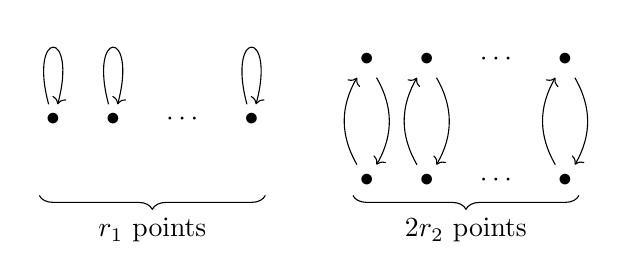
\begin{tikzpicture}
    \matrix(m)[matrix of math nodes, row sep=1em, column sep=1em,
    text height=1ex, text depth=0.2ex]{
      ~ & ~ & ~ & ~ & ~ & \bullet & \bullet & \cdots & \bullet \\
      \bullet & \bullet & \cdots & \bullet \\
      ~ & ~ & ~ & ~ & ~ & \bullet & \bullet & \cdots & \bullet \\};

    \draw[->] (m-2-1) edge[loop above,min distance=10mm] (m-2-1);
    \draw[->] (m-2-2) edge[loop above,min distance=10mm] (m-2-2);
    \draw[->] (m-2-4) edge[loop above,min distance=10mm] (m-2-4);

    \draw[->] (m-1-6) edge[bend left] (m-3-6);
    \draw[->] (m-1-7) edge[bend left] (m-3-7);
    \draw[->] (m-1-9) edge[bend left] (m-3-9);

    \draw[->] (m-3-6) edge[bend left] (m-1-6);
    \draw[->] (m-3-7) edge[bend left] (m-1-7);
    \draw[->] (m-3-9) edge[bend left] (m-1-9);

    \draw [decorate,decoration={brace,amplitude=5pt,mirror}] ($(m-3-1)+(-0.5em,-0.5em)$) -- ($(m-3-4)+(0.5em,-0.5em)$);
    \draw [decorate,decoration={brace,amplitude=5pt,mirror}] ($(m-3-6)+(-0.5em,-0.5em)$) -- ($(m-3-9)+(0.5em,-0.5em)$);

    \draw ($(m-3-1)!.5!(m-3-4)$) node[yshift=-2em,anchor=base] {$r_1$ points};
    \draw ($(m-3-6)!.5!(m-3-9)$) node[yshift=-2em,anchor=base] {$2 r_2$ points};
  \end{tikzpicture} \]

  The complex $R\Gamma_c (X (\CC), \RR (n))$ consists of a single $G_\RR$-module
  in degree $0$ given by
  $$\RR (n)^{\oplus r_1} \oplus (\RR (n) \oplus \RR (n))^{\oplus r_2},$$
  with the action of $G_\RR$ on the first summand $\RR (n)^{\oplus r_1}$ via the
  complex conjugation and the action on the second summand
  $(\RR (n) \oplus \RR (n))^{\oplus r_2}$ via
  $(x,y) \mapsto (\overline{y}, \overline{x})$. The corresponding real space of
  fixed points has dimension
  \[ \dim_\RR H^0_c (G_\RR, X (\CC), \RR (n)) = \begin{cases}
      r_2, & n \text{ odd},\\
      r_1 + r_2, & n \text{ even},\\
    \end{cases} \]
  which indeed coincides with the vanishing order of the Dedekind zeta function
  $\zeta (X,s) = \zeta_F (s)$ at $s = n < 0$.

  On the motivic cohomology side \cite[Proposition~4.14]{Geisser-2017}, for
  $n < 0$ the groups $H^i (X_\et, \ZZ^c (n)) = H^{i+2} (X_\et, \ZZ (1-n))$ are
  finite, except for $i = -1$, where
  \[ \rk_\ZZ H^{-1} (X_\et, \ZZ^c (n)) =
    \rk_\ZZ H^1 (X_\et, \ZZ (1-n)) = \begin{cases}
      r_2, & n \text{ odd},\\
      r_1 + r_2, & n \text{ even}.
    \end{cases} \]
\end{example}

\begin{example}
  Suppose that $X$ is a variety over a finite field $\FF_q$. Then the vanishing
  order conjecture is not very interesting, because the formula yields
  \begin{align*}
    \ord_{s=n} \zeta (X,s) & = \sum_{i \in \ZZ} (-1)^i \dim_\RR H^i_c (X(\CC), \RR (n))^{G_\RR} \\
                           & = \sum_{i \in \ZZ} (-1)^{i+1} \rk_\ZZ H^i (X_\et, \ZZ^c (n)) = 0,
  \end{align*}
  since $X (\CC) = \emptyset$, and also because $\mathbf{L}^c (X_\et, n)$
  implies $\rk_\ZZ H^i (X_\et, \ZZ^c (n)) = 0$ in the case of varieties over
  finite fields, as observed in
  \cite[Proposition~4.2]{Beshenov-Weil-etale-1}. Therefore, the conjecture
  simply asserts that $\zeta (X,s)$ has no zeros or poles at $s = n < 0$.
  This is indeed the case. We have $\zeta (X,s) = Z (X,q^{-s})$, where
  $$Z (X,t) = \exp \Bigl(\sum_{k\ge 1} \frac{\# X (\FF_{q^k})}{k}\,t^k\Bigr)$$
  is the Hasse--Weil zeta function. According to Deligne's work on Weil's
  conjectures \cite{Deligne-Weil-II}, the zeros and poles of $Z (X,s)$ satisfy
  $|s| = q^{-w/2}$, where $0 \le w \le 2 \dim X$ (see
  e.g. \cite[pp.\,26--27]{Katz-1994}). In particular, $q^{-s}$ for $s = n < 0$
  is neither a zero nor a pole of $Z (X,s)$.

  We also note that our definition of $H^i_\Wc (X, \ZZ(n))$, and pretty much
  everything said above, only makes sense for $n < 0$. Already for $n = 0$, for
  example, the zeta function of a smooth projective curve $X/\FF_q$ has a simple
  pole at $s = 0$.
\end{example}

\begin{example}
  Let $X = E$ be an integral model of an elliptic curve over $\QQ$. Then, as a
  consequence of the modularity theorem
  (Wiles--Breuil--Conrad--Diamond--Taylor), it is known that $\zeta (E,s)$
  admits a meromorphic continuation satisfying the functional equation with the
  $\Gamma$-factors discussed in Remark~\ref{rmk:archimedian-euler-factor}.
  In this particular case $\ord_{s=n} \zeta (E,s) = 0$ for all $n < 0$. This is
  consistent with the fact that
  $\chi (R\Gamma_c (G_\RR, E (\CC), \RR (n))) = 0$.

  Indeed, the equivariant cohomology groups $H^i_c (E (\CC), \RR (n))^{G_\RR}$
  are the following:
  \begin{center}
    \renewcommand{\arraystretch}{1.5}
    \begin{tabular}{rccc}
      \hline
      & $i = 0$ & $i = 1$ & $i = 2$ \\
      \hline
      $n$ even: & $\RR$ & $\RR$ & $0$ \\
      $n$ odd: & $0$ & $\RR$ & $\RR$ \\
      \hline
    \end{tabular}
  \end{center}
  ---see, for example, the calculation in \cite[Lemma~A.6]{Siebel-2019}.
\end{example}

%%%%%%%%%%%%%%%%%%%%%%%%%%%%%%%%%%%%%%%%%%%%%%%%%%%%%%%%%%%%%%%%%%%%%%%%%%%%%%%%

\section{Special value conjecture~$\mathbf{C} (X,n)$}
\label{sec:special-value-conjecture}

\begin{definition}
  We define a morphism of complexes
  \[ \smile\theta\colon R\Gamma_\Wc (X,\ZZ(n)) \otimes \RR \to
    R\Gamma_\Wc (X,\ZZ(n)) [1] \otimes \RR \]
  using the splitting \cite[Proposition~7.13]{Beshenov-Weil-etale-1}
  \[ R\Gamma_\Wc (X, \RR (n)) \cong
    \RHom (R\Gamma (X_\et, \ZZ^c (n)), \RR) [-1] \oplus
    R\Gamma_c (G_\RR, X (\CC), \RR (n)) [-1] \]
  as follows:
  \[ \begin{tikzcd}
      R\Gamma_\Wc (X, \RR(n)) \ar{d}{\cong}\ar[dashed]{r}{\smile\theta} & R\Gamma_\Wc (X, \RR(n)) [1]\ar{d}{\cong} \\
      \RHom (R\Gamma (X_\et, \ZZ^c (n)), \RR) [-1] & \RHom (R\Gamma (X_\et, \ZZ^c (n)), \RR) \\[-2em]
      \oplus & \oplus \\[-2em]
      R\Gamma_c (G_\RR, X (\CC), \RR (n)) [-1]\ar{uur}[description]{Reg_{X,n}^\vee} & R\Gamma_c (G_\RR, X (\CC), \RR (n))
    \end{tikzcd} \]
\end{definition}

\begin{lemma}
  \label{lemma:smile-theta}
  Assuming Conjectures $\mathbf{L}^c (X_\et,n)$ and $\mathbf{B} (X,n)$, the
  morphism $\smile\theta$ induces a long exact sequence of finite dimensional
  real vector spaces
  \[ \cdots \to H^{i-1}_\Wc (X, \RR (n))
    \xrightarrow{\smile\theta}
    H^i_\Wc (X, \RR (n))
    \xrightarrow{\smile\theta}
    H^{i+1}_\Wc (X, \RR (n)) \to \cdots \]

  \begin{proof}
    We obtain a sequence
    \[ \begin{tikzcd}[column sep=1em]
        \cdots\ar{r} & H^i_\Wc (X, \RR(n))\ar{d}{\cong}\ar[dashed]{r}{\smile\theta} & H^{i+1}_\Wc (X, \RR(n))\ar{d}{\cong} \ar{r} & \cdots \\
        & \Hom (H^{-i-1} (X_\et, \ZZ^c (n)), \RR) & \Hom (H^{-i-2} (X_\et, \ZZ^c (n)), \RR) \\[-2em]
        \cdots & \oplus & \oplus & \cdots \\[-2em]
        & H_c^{i-1} (G_\RR, X (\CC), \RR (n))\ar{uur}[description]{\cong} & H_c^i (G_\RR, X (\CC), \RR (n))
      \end{tikzcd} \]
    The diagonal arrows are isomorphisms according to $\mathbf{B} (X,n)$,
    so the sequence is exact.
  \end{proof}
\end{lemma}

The Weil-\'{e}tale complex $R\Gamma_\Wc (X, \ZZ(n))$ is defined in
\cite[\S 7]{Beshenov-Weil-etale-1} up to a \emph{non-unique} isomorphism in the
derived category $\mathbf{D} (\ZZ)$ via a distinguished triangle
\begin{equation}
  \label{eqn:triangle-defining-RGamma-Wc}
  R\Gamma_\Wc (X, \ZZ(n)) \to R\Gamma_\fg (X,\ZZ(n)) \xrightarrow{i_\infty}
  R\Gamma_c (G_\RR, X (\CC), \ZZ (n)) \to [1]
\end{equation}
This is rather awkward, and there should be a better, more canonical
construction of $R\Gamma_\Wc (X, \ZZ(n))$. For our purposes, however, this is
not much of a problem, since the special value conjecture is not formulated in
terms of $R\Gamma_\Wc (X, \ZZ (n))$, but in terms of its determinant
$\det_\ZZ R\Gamma_\Wc (X, \ZZ(n))$ (see Appendix~\ref{app:determinants}), which
is well-defined.

\begin{lemma}
  \label{lemma:determinant-of-RGamma-Wc-well-defined}
  The determinant $\det_\ZZ R\Gamma_\Wc (X, \ZZ(n))$ is defined up to a
  canonical isomorphism.

  \begin{proof}
    Two different choices for the mapping fiber in
    \eqref{eqn:triangle-defining-RGamma-Wc} yield an isomorphism of
    distinguished triangles
    \[ \begin{tikzcd}
        R\Gamma_\Wc (X, \ZZ(n)) \ar{r}\ar{d}{f}[swap]{\cong} & R\Gamma_\fg (X,\ZZ(n)) \ar{r}{i_\infty}\ar{d}{id} & R\Gamma_c (G_\RR, X (\CC), \ZZ (n)) \ar{r}\ar{d}{id} & {[1]}\ar{d}{f}[swap]{\cong} \\
        R\Gamma_\Wc (X, \ZZ(n))' \ar{r} & R\Gamma_\fg (X,\ZZ(n)) \ar{r}{i_\infty} & R\Gamma_c (G_\RR, X (\CC), \ZZ (n)) \ar{r} & {[1]}
      \end{tikzcd} \]
    The idea is to use functoriality of determinants with respect to
    isomorphisms of distinguished triangles
    (Proposition~\ref{prop:det-and-isos-of-triangles}). The only technical problem
    is that whenever $X (\RR) \ne \emptyset$, the complexes
    $R\Gamma_\fg (X,\ZZ(n))$ and $R\Gamma_c (G_\RR, X (\CC), \ZZ (n))$ are not
    perfect, but may have finite $2$-torsion in $H^i (-)$ for arbitrarily big
    $i$ (in \cite{Beshenov-Weil-etale-1} we called such complexes
    \textbf{almost perfect}). On the other hand, the determinants are defined
    only for perfect complexes. Fortunately, $H^i (i_\infty^*)$ is an
    isomorphism for $i \gg 0$ by the boundedness of $H^i_\Wc (X, \ZZ(n))$
    \cite[Proposition~7.12]{Beshenov-Weil-etale-1}, so that for $m$ big enough
    we can take the corresponding canonical truncations $\tau_{\le m}$:
    \[ \begin{tikzcd}[row sep=1.5em, column sep=0.75em, font=\small]
        \tau_{\le m} R\Gamma_\Wc (X, \ZZ(n)) \ar{r}\ar{d}{\cong} & \tau_{\le m} R\Gamma_\fg (X,\ZZ(n)) \ar{r}\ar{d} & \tau_{\le m} R\Gamma_c (G_\RR, X (\CC), \ZZ (n)) \ar{r}\ar{d} & {[1]}\ar{d}{\cong} \\
        R\Gamma_\Wc (X, \ZZ(n)) \ar{r}\ar{d} & R\Gamma_\fg (X,\ZZ(n)) \ar{r}{i_\infty}\ar{d} & R\Gamma_c (G_\RR, X (\CC), \ZZ (n)) \ar{r}\ar{d} & {[1]}\ar{d} \\
        0 \ar{r}\ar{d} & \tau_{\ge m+1} R\Gamma_\fg (X,\ZZ(n)) \ar{r}{\cong}\ar{d} & \tau_{\ge m+1} R\Gamma_c (G_\RR, X (\CC), \ZZ (n)) \ar{r}\ar{d} & 0\ar{d} \\
        {[1]} \ar{r} & {[1]} \ar{r} & {[1]} \ar{r} & {[2]}
      \end{tikzcd} \]

    The truncations give us (rotating the triangles)
    \[ \begin{tikzcd}[column sep=1em,font=\small]
        \tau_{\le m} R\Gamma_c (G_\RR, X (\CC), \ZZ (n))[-1] \ar{r}\ar{d}{id} & R\Gamma_\Wc (X, \ZZ (n))\ar{d}{f}[swap]{\cong}\ar{r} & \tau_{\le m} R\Gamma_\fg (X,\ZZ(n)) \ar{d}{id}\ar{r} & {[0]} \ar{d}{id} \\
        \tau_{\le m} R\Gamma_c (G_\RR, X (\CC), \ZZ (n))[-1] \ar{r} & R\Gamma_\Wc (X, \ZZ (n))' \ar{r} & \tau_{\le m} R\Gamma_\fg (X,\ZZ(n)) \ar{r} & {[0]}
      \end{tikzcd} \]
    By Proposition~\ref{prop:det-and-isos-of-triangles}, we have a commutative
    diagram
    \[ \begin{tikzcd}
        \begin{array}{c} \det_\ZZ \tau_{\le m} R\Gamma_c (G_\RR, X (\CC), \ZZ (n))[-1] \\ \otimes \\ \det_\ZZ \tau_{\le m} R\Gamma_\fg (X,\ZZ(n)) \end{array} \ar{r}{i}[swap]{\cong} \ar{d}{id} & \det_\ZZ R\Gamma_\Wc (X,\ZZ(n)) \ar{d}{\det_\ZZ (f)}[swap]{\cong} \\
        \begin{array}{c} \det_\ZZ \tau_{\le m} R\Gamma_c (G_\RR, X (\CC), \ZZ (n))[-1] \\ \otimes \\ \det_\ZZ \tau_{\le m} R\Gamma_\fg (X, \ZZ (n)) \end{array} \ar{r}{i'}[swap]{\cong} & \det_\ZZ R\Gamma_\Wc (X,\ZZ(n))
      \end{tikzcd} \]
    so that $\det_\ZZ (f) = i'\circ i^{-1}$.
  \end{proof}
\end{lemma}

\begin{lemma}
  The non-canonical splitting
  \[ R\Gamma_\Wc (X, \QQ(n)) \cong
    \RHom (R\Gamma (X_\et, \ZZ^c (n)), \QQ) [-1] \oplus
    R\Gamma_c (G_\RR, X (\CC), \QQ (n)) [-1] \]
  from \cite[Proposition~7.13]{Beshenov-Weil-etale-1} yields a canonical
  isomorphism of determinants
  \[ \det_\QQ R\Gamma_\Wc (X, \QQ(n)) \cong
    \begin{array}{c}
      \det_\QQ \RHom (R\Gamma (X_\et, \ZZ^c (n)), \QQ) [-1] \\
      \otimes_\QQ \\
      \det_\QQ R\Gamma_c (G_\RR, X (\CC), \QQ (n)) [-1]
    \end{array} \]

  \begin{proof}
    This is similar to the previous lemma; in fact, after tensoring with $\QQ$,
    we obtain perfect complexes of $\QQ$-vector spaces, so the truncations are
    no longer needed. By \cite[Proposition~7.4]{Beshenov-Weil-etale-1} we have
    $i_\infty^* \otimes \QQ = 0$, so there is an isomorphism of triangles
    \begin{equation}
      \label{eqn:splitting-of-RGamma-Wc-triangles}
      \begin{tikzcd}[row sep=1em]
        R\Gamma_c (G_\RR, X (\CC), \QQ (n)) [-1] \ar{r}{id}\ar{d} & R\Gamma_c (G_\RR, X (\CC), \QQ (n)) [-1]\ar{d} \\
        R\Gamma_\Wc (X, \QQ(n)) \ar[dashed]{r}{f}[swap]{\cong}\ar{d} & \begin{array}{c} \RHom (R\Gamma (X_\et, \ZZ^c (n)), \QQ) [-1] \\ \oplus \\ R\Gamma_c (G_\RR, X (\CC), \QQ (n)) [-1] \end{array}\ar{d} \\
        R\Gamma_\fg (X, \QQ(n)) \ar{r}{g\otimes \QQ}[swap]{\cong}\ar{d} & \RHom (R\Gamma (X_\et, \ZZ^c (n)), \QQ) [-1] \ar{d} \\
        R\Gamma_c (G_\RR, X (\CC), \QQ (n)) \ar{r}{id} & R\Gamma_c (G_\RR, X (\CC), \QQ (n))
      \end{tikzcd}
    \end{equation}
    Here the third horizontal arrow comes from the triangle defining
    $R\Gamma_\fg (X, \ZZ(n))$
    \begin{multline*}
      \RHom (R\Gamma (X_\et, \ZZ^c (n)), \QQ) [-2] \xrightarrow{\alpha_{X,n}}
      R\Gamma_c (X_\et, \ZZ (n)) \to
      R\Gamma_\fg (X, \ZZ(n)) \\
      \xrightarrow{g} \RHom (R\Gamma (X_\et, \ZZ^c (n)), \QQ) [-1]
    \end{multline*}
    tensored with $\QQ$ (see \cite[Proposition~5.7]{Beshenov-Weil-etale-1}).
    The distinguished column on the right-hand side of
    \eqref{eqn:splitting-of-RGamma-Wc-triangles} is the direct sum
    \[ \begin{tikzcd}[row sep=1.5em]
        R\Gamma_c (G_\RR, X (\CC), \QQ (n)) [-1]\ar{d}{id} &[-2em] &[-2em] 0\ar{d} \\
        R\Gamma_c (G_\RR, X (\CC), \QQ (n)) [-1]\ar{d} & \oplus & \RHom (R\Gamma (X_\et, \ZZ^c (n)), \QQ) [-1]\ar{d}{id} \\
        0 \ar{d} & & \RHom (R\Gamma (X_\et, \ZZ^c (n)), \QQ) [-1] \ar{d} \\
        R\Gamma_c (G_\RR, X (\CC), \QQ (n)) & & 0
      \end{tikzcd} \]
    The splitting isomorphism $f$ in
    \eqref{eqn:splitting-of-RGamma-Wc-triangles} is not canonical at
    all. However, after taking the determinants, we obtain a commutative diagram
    (see Proposition~\ref{prop:det-and-isos-of-triangles})
    \[ \begin{tikzcd}[column sep=1em, font=\small]
        \begin{array}{c} \det_\QQ R\Gamma_c (G_\RR, X (\CC), \QQ (n)) [-1] \\ \otimes_\QQ \\ \det_\QQ R\Gamma_\fg (X, \QQ(n)) \end{array} \ar{r}{i}[swap]{\cong} \ar{d}{id \otimes \det_\ZZ (g\otimes \QQ)}[swap]{\cong} & \det_\QQ R\Gamma_\Wc (X, \QQ(n)) \ar{d}{\det_\ZZ (f)}[swap]{\cong}\ar[dashed]{dl}{\cong} \\
        \begin{array}{c} \det_\QQ R\Gamma_c (G_\RR, X (\CC), \QQ (n)) [-1] \\ \otimes_\QQ \\ \det_\QQ \RHom (R\Gamma (X_\et, \ZZ^c (n)), \QQ) [-1] \end{array} \ar{r}{i'}[swap]{\cong} & \det_\QQ \left(\!\!\!\begin{array}{c} \RHom (R\Gamma (X_\et, \ZZ^c (n)), \QQ) [-1] \\ \oplus \\ R\Gamma_c (G_\RR, X (\CC), \QQ (n)) [-1] \end{array}\!\!\!\right)
      \end{tikzcd} \]
    The dashed diagonal arrow is the desired canonical isomorphism.
  \end{proof}
\end{lemma}

\begin{definition}
  Given an arithmetic scheme $X$ and $n < 0$, assume
  Conjectures~$\mathbf{L}^c (X_\et, n)$ and $\mathbf{B} (X,n)$. Consider the
  quasi-isomorphism
  \begin{multline}\small
    \label{eqn:definition-of-lambda}
    \left(\!\!\!\begin{array}{c} R\Gamma_c (G_\RR, X (\CC), \RR (n)) [-2] \\ \oplus \\ R\Gamma_c (G_\RR, X (\CC), \RR (n)) [-1] \end{array}\!\!\!\right)
    \xrightarrow[\cong]{Reg_{X,n}^\vee [-1] \oplus id}
    \left(\!\!\!\begin{array}{c} \RHom (R\Gamma (X_\et, \ZZ^c (n)), \RR) [-1] \\ \oplus \\ R\Gamma_c (G_\RR, X (\CC), \RR (n)) [-1] \end{array}\!\!\!\right) \\
    \\
    \xrightarrow[\cong]{\text{split}} R\Gamma_\Wc (X, \RR (n))
  \end{multline}
  Note that the first complex has determinant
  \[ \det_\RR \left(\!\!\begin{array}{c} R\Gamma_c (G_\RR, X (\CC), \RR (n)) [-2] \\ \oplus \\ R\Gamma_c (G_\RR, X (\CC), \RR (n)) [-1] \end{array}\!\!\right) \cong
    \begin{array}{c} \det_\RR R\Gamma_c (G_\RR, X (\CC), \RR (n)) \\ \otimes_\RR \\ (\det_\RR R\Gamma_c (G_\RR, X (\CC), \RR (n)))^{-1} \end{array} \cong \RR, \]
  and for the last complex, by the compatibility with base change, we have a
  canonical isomorphism
  \[ \det_\RR R\Gamma_\Wc (X, \RR (n)) \cong
    (\det_\ZZ R\Gamma_\Wc (X, \ZZ (n))) \otimes \RR. \]
  Therefore, after taking the determinants, the quasi-isomorphism
  \eqref{eqn:definition-of-lambda} induces a canonical isomorphism
  \begin{equation}
    \label{eqn:morphism-lambda}
    \lambda = \lambda_{X,n}\colon \RR \xrightarrow{\cong}
    (\det_\ZZ R\Gamma_\Wc (X, \ZZ (n))) \otimes \RR.
  \end{equation}
\end{definition}

\begin{remark}
  An equivalent way to define $\lambda$ is
  \begin{multline*}
    \lambda\colon \RR \xrightarrow{\cong}
    \bigotimes_{i\in \ZZ} (\det_\RR H^i_\Wc (X, \RR (n)))^{(-1)^i} \\
    \xrightarrow{\cong} \Bigl(\bigotimes_{i\in \ZZ} (\det_\ZZ H^i_\Wc (X, \ZZ (n)))^{(-1)^i}\Bigr) \otimes \RR \\
    \xrightarrow{\cong} (\det_\ZZ R\Gamma_\Wc (X, \ZZ (n))) \otimes \RR,
  \end{multline*}
  where the first isomorphism comes from Lemma~\ref{lemma:smile-theta}.
\end{remark}

We are ready to state the main conjecture of this paper. The determinant
$\det_\ZZ R\Gamma_\Wc (X, \ZZ (n)))$ is a free $\ZZ$-module of rank $1$, and the
isomorphism \eqref{eqn:morphism-lambda} canonically embeds it in $\RR$. We
conjecture that this embedding gives the special value of $\zeta (X,s)$ at
$s = n$ in the following sense.

\begin{conjecture}
  $\mathbf{C} (X,n)$: let $X$ be an arithmetic scheme and $n < 0$ a strictly
  negative integer. Assuming Conjectures~$\mathbf{L}^c (X_\et, n)$,
  $\mathbf{B} (X,n)$ and the meromorphic continuation of $\zeta (X,s)$ around
  $s = n < 0$, the corresponding special value is determined up to sign by
  \[ \lambda (\zeta^* (X,n)^{-1}) \cdot \ZZ =
    \det_\ZZ R\Gamma_\Wc (X, \ZZ (n)), \]
  where $\lambda$ is the canonical isomorphism \eqref{eqn:morphism-lambda}.
\end{conjecture}

\begin{remark}
  This conjecture is similar to \cite[Conjecture~5.12]{Flach-Morin-2018}.
  When $X$ is proper and regular, the above conjecture is the same as the
  special value conjecture of Flach and Morin, which for $n \in \ZZ$ reads
  \begin{equation}
    \label{eqn:FM-special-value}
    \lambda_\infty \Bigl(\zeta^* (X,n)^{-1} \cdot C (X,n) \cdot \ZZ\Bigr) =
    \Delta (X/\ZZ, n).
  \end{equation}
  Here the fundamental line $\Delta (X/\ZZ,n)$ is defined via
  \[ \Delta (X/\ZZ,n) \dfn
    \det_\ZZ R\Gamma_\Wc (X, \ZZ(n)) \otimes
    \det_\ZZ R\Gamma_\dR (X/\ZZ)/\Fil^n. \]
  If $n < 0$, then
  $\Delta (X/\ZZ,n) = \det_\ZZ R\Gamma_\Wc (X, \ZZ(n))$. Moreover, $C (X,n)$ is
  a rational number, defined via $\prod_p |c_p (X,n)|_p$.
  Here $c_p (X,n) \in \QQ_p^\times/\ZZ_p^\times$ are the local factors
  described in \cite[\S 5.4]{Flach-Morin-2018}, but
  \cite[Proposition~5.8]{Flach-Morin-2018} states that if $n \le 0$, then
  $c_p (X,n) \equiv 1 \pmod{\ZZ_p^\times}$ for all $p$. Therefore, $C (X,n) = 1$
  in our situation. Finally, the trivialization isomorphism $\lambda_\infty$ is
  defined exactly as our $\lambda$. Therefore, \eqref{eqn:FM-special-value} for
  $n < 0$ agrees with Conjecture~$\mathbf{C} (X,n)$.

  Flach and Morin prove that their conjecture is consistent with the Tamagawa
  number conjecture of Bloch--Kato--Fontaine--Perrin-Riou
  \cite{Fontaine-Perrin-Riou-1994}; see \cite[\S 5.6]{Flach-Morin-2018} for the
  details.
\end{remark}

\begin{remark}
  Some canonical isomorphisms of determinants involve multiplication by $\pm 1$,
  so it is no surprise that the resulting conjecture is stated up to sign
  $\pm 1$. This is not a major problem, however, since the sign can be recovered
  from the (conjectural) functional equation.
\end{remark}

%%%%%%%%%%%%%%%%%%%%%%%%%%%%%%%%%%%%%%%%%%%%%%%%%%%%%%%%%%%%%%%%%%%%%%%%%%%%%%%%

\section{Case of varieties over finite fields}
\label{sec:finite-fields}

For varieties over finite fields, our special value conjecture corresponds to
the conjectures studied by Geisser in
\cite{Geisser-2004,Geisser-2006,Geisser-2010-arithmetic-homology}.

\begin{proposition}
  \label{prop:C(X,n)-over-finite-fields}
  If $X/\FF_q$ is a variety over a finite field, then assuming
  $\mathbf{L}^c (X_\et,n)$, the special value conjecture
  $\mathbf{C} (X,n)$ is equivalent to
  \begin{align}
    \label{eqn:special-value-for-X/Fq}
    \notag \zeta^* (X,n) & = \pm \prod_{i \in \ZZ} |H_\Wc^i (X, \ZZ(n))|^{(-1)^i} \\
                         & = \pm \prod_{i \in \ZZ} |H^i (X_\et, \ZZ^c (n))|^{(-1)^i} \\
    \notag & = \pm \prod_{i \in \ZZ} |H_i^c (X_\ar, \ZZ (n))|^{(-1)^{i+1}},
  \end{align}
  where $H_i^c (X_\ar, \ZZ (n))$ are Geisser's arithmetic homology groups
  defined in \cite{Geisser-2010-arithmetic-homology}.

  \begin{proof}
    Assuming $\mathbf{L}^c (X_\et,n)$, thanks to
    \cite[Proposition~7.7]{Beshenov-Weil-etale-1} we have
    \[ H^i_\Wc (X, \ZZ (n)) \cong
      \Hom (H^{2-i} (X_\et, \ZZ^c (n)), \QQ/\ZZ) \cong
      \Hom (H_{i-1}^c (X_\ar, \ZZ (n)), \QQ/\ZZ). \]
    The involved cohomology groups are finite and vanish for $|i| \gg 0$
    (see \cite[Proposition~4.2]{Beshenov-Weil-etale-1}), and therefore by
    \ref{lemma:determinant-for-torsion-cohomology}, the determinant is given by
    \[ \begin{tikzcd}[row sep=0.75em, column sep=0pt]
        \det_\ZZ R\Gamma_\Wc (X, \ZZ (n)) \ar[equals]{d} & \subset & \det_\ZZ R\Gamma_\Wc (X, \ZZ (n)) \otimes \QQ \ar[equals]{d} \\
        \frac{1}{m}\ZZ & \subset & \QQ
      \end{tikzcd} \]
    where
    \[ m = \prod_{i \in \ZZ} |H_\Wc^i (X, \ZZ(n))|^{(-1)^i}. \qedhere \]
  \end{proof}
\end{proposition}

\begin{remark}
  Formulas similar to \eqref{eqn:special-value-for-X/Fq} were suggested long
  time ago by Lichtenbaum in \cite{Lichtenbaum-1984}.
\end{remark}

\begin{theorem}
  \label{thm:C(X,n)-over-finite-fields}
  Let $X/\FF_q$ be a variety over a finite field satisfying
  $\mathbf{L}^c (X_\et, n)$ for $n < 0$. Then Conjecture~$\mathbf{C} (X,n)$
  holds.
\end{theorem}

We note that \eqref{prop:C(X,n)-over-finite-fields} is equivalent to the special
value formula that appears in
\cite[Theorem~4.5]{Geisser-2010-arithmetic-homology}.
Conjecture~$\mathbf{P}_0 (X)$ in the statement of
\cite[Theorem~4.5]{Geisser-2010-arithmetic-homology} is implied by our
Conjecture~$\mathbf{L}^c (X_\et,n)$ thanks to
\cite[Proposition~4.1]{Geisser-2010-arithmetic-homology}. Geisser's proof
eventually reduces to \cite{Milne-1986}, but for our case of $s = n < 0$, the
situation is easier, and we can give a more direct explanation, using earlier
results from \cite{Bayer-Neukirch-1978} regarding Grothendieck's trace formula.

\begin{proof}
  In this case the conjecture reduces to
  $$\zeta (X,n) = \prod_{i \in \ZZ} |H^i (X_\et, \ZZ^c (n))|^{(-1)^i}.$$

  By duality \cite[Theorem~I]{Beshenov-Weil-etale-1}, we have
  $$|H^{2-i} (X_\et, \ZZ^c (n))| = |H^i_c (X_\et, \ZZ (n))|,$$
  where
  \[ \ZZ (n) \dfn
    \bigoplus_{\ell \ne p} \QQ_\ell/\ZZ_\ell (n) [-1] \dfn
    \bigoplus_{\ell \ne p} \mu_{\ell^\infty}^{\otimes n} [-1] \dfn
    \bigoplus_{\ell \ne p} \varinjlim_r \mu_{\ell^r}^{\otimes n} [-1]. \]
  Now $H^i_c (X_\et, \QQ_\ell (n)) = 0$ for $n < 0$, and therefore
  $H^i_c (X_\et, \ZZ_\ell (n)) \cong
  H^{i-1}_c (X_\et, \QQ_\ell/\ZZ_\ell (n))$.
  This means that our conjectural formula can be written as
  \[ \zeta (X,n) =
    \prod_{\ell \ne p} \prod_{i \in \ZZ} |H^i_c (X_\et, \ZZ_\ell (n))|^{(-1)^i}. \]

  Grothendieck's trace formula (see \cite{Grothendieck-FL} or
  \cite[Rapport]{SGA4-1-2}) reads
  \[ Z (X,t) =
    \prod_{i \in \ZZ} \det \bigl(1 - tF \bigm| H^i_c (\overline{X}, \QQ_\ell)\bigr)^{(-1)^{i+1}}. \]
  Here $\overline{X} \dfn X \times_{\Spec \FF_q} \overline{\FF}_q$, and $F$
  is the Frobenius acting on $H^i_c (\overline{X}, \QQ_\ell)$. Substituting
  $t = q^{-n}$,
  \[ \zeta (X,n) =
    \prod_{i \in \ZZ} \det \bigl(1 - q^{-n} F \bigm| H^i_c (\overline{X}, \QQ_\ell)\bigr)^{(-1)^{i+1}}. \]
  Then following the proof of \cite[Theorem~(3.1)]{Bayer-Neukirch-1978}, we
  obtain for each $\ell \ne p$
  \begin{equation}
    \label{eqn:bayer-neukirch}
    |\zeta (X,n)|_\ell =
    \prod_{i \in \ZZ} |H^i_c (X, \ZZ_\ell (n))|^{(-1)^{i+1}}.
  \end{equation}

  On the other hand, for $n < 0$ we have $|\zeta (X,n)|_p = 1$. This fact can
  be justified, without assuming that $X$ is smooth or projective,
  for instance, using the trace formula for rigid cohomology
  \cite[p.\,1446]{Kedlaya-2006}, which gives
  $Z (X,t) = \prod_i P_i (t)^{(-1)^{i+1}}$, where $P_i (t) \in \ZZ[t]$ and
  $P_i (0) = 1$. In particular, $P_i (q^{-n}) \equiv 1 \pmod{p}$.
  We conclude that the product formula gives from \eqref{eqn:bayer-neukirch}
  \[ \zeta (X,n) =
    \prod_{\ell \ne p} \prod_{i \in \ZZ} |H^i_c (X, \ZZ_\ell (n))|^{(-1)^i}, \]
  which is precisely our special value formula.
\end{proof}

\begin{remark}
  The fact that $|\zeta (X,n)|_p = 1$ observed in the above argument explains
  why Weil-\'{e}tale cohomology ignores the $p$-primary part in a sense.
\end{remark}

Let us consider a couple of particular examples to see how the special value
conjecture works. It is to be noted that for a general arithmetic scheme $X$,
calculating the motivic cohomology $H^i (X_\et, \ZZ^c (n))$ (and therefore our
Weil-\'{e}tale cohomology $H^i_\Wc (X, \ZZ(n))$) is by no means a trivial task. The
finite generation of $H^i (X_\et, \ZZ^c (n))$ is only known for particular cases
(see \cite[\S 8]{Beshenov-Weil-etale-1}), and calculating the torsion part,
which bears the arithmetic information, is even more difficult. Similarly, an
explicit calculation of the regulator map $Reg_{X,n}$ is highly
nontrivial. Therefore, for the moment we give some toy examples over finite
fields.

\begin{example}
  \label{example:C(X,n)-for-Spec-Fq}
  If $X = \Spec \FF_q$, then $\zeta (X,s) = \frac{1}{1 - q^{-s}}$. In this case
  for $n < 0$ we obtain
  \begin{equation}
    \label{eqn:motivic-cohomology-of-Fq}
    H^i (\Spec \FF_{q,\et}, \ZZ^c (n)) = H^i (\Spec \FF_{q,\et}, \ZZ (-n)) =
    \begin{cases}
      \ZZ/(q^{-n} - 1), & i = 1, \\
      0, & i \ne 1
    \end{cases}
  \end{equation}
  (see for instance \cite[Example~4.2]{Geisser-2017}).
  Therefore, the formula \eqref{eqn:special-value-for-X/Fq} indeed recovers
  $\zeta (X,n)$ up to sign.

  Similarly, replacing $\Spec \FF_q$ with $\Spec \FF_{q^m}$, viewed as a variety
  over $\FF_q$, we have $\zeta (\Spec \FF_{q^m},s) = \zeta (\Spec \FF_q, ms)$,
  and \eqref{eqn:motivic-cohomology-of-Fq} also changes accordingly.
\end{example}

\begin{example}
  Consider $X = \PP^1_{\FF_q}/(0\sim 1)$, or equivalently, a nodal cubic.
  The zeta function is $\zeta (X,s) = \frac{1}{1 - q^{1-s}}$.  We can calculate
  the groups $H^i (X_\et, \ZZ^c (n))$ using the blowup square
  \[ \begin{tikzcd}
      \Spec \FF_q \sqcup \Spec \FF_q \ar{r}\ar{d}\tikzpb & \PP^1_{\FF_q} \ar{d} \\
      \Spec \FF_q \ar{r} & X
    \end{tikzcd} \]
  This is similar to \cite[\S 8, Example~2]{Geisser-2006}. Geisser uses
  eh-topology and long exact sequences associated to abstract blowup squares
  \cite[Proposition~3.2]{Geisser-2006}. In our case, the same works, since
  according to \cite[Theorem~I]{Beshenov-Weil-etale-1}, one has
  $H^i (X_\et, \ZZ^c (n)) \cong \Hom (H^{2-i}_c (X_\et, \ZZ (n)),\QQ/\ZZ)$,
  where $\ZZ (n) = \varinjlim_{p\nmid m} \mu_m^{\otimes n} [-1]$, and
  for such sheaves \'{e}tale cohomology and eh-cohomology agree by
  \cite[Theorem~3.6]{Geisser-2006}.

  Using the projective bundle formula, we calculate from
  \eqref{eqn:motivic-cohomology-of-Fq}
  \[ H^i (\PP^1_{\FF_q,\et}, \ZZ^c (n)) = \begin{cases}
      \ZZ/(q^{1-n} - 1), & i = -1, \\
      \ZZ/(q^{-n} - 1), & i = +1, \\
      0, & i \ne \pm 1.
    \end{cases} \]
  Following the same argument from \cite[\S 8, Example~2]{Geisser-2006},
  the short exact sequences
  \[ 0 \to H^i (\PP^1_{\FF_q,\et}, \ZZ^c (n)) \to
    H^i (X_\et, \ZZ^c (n)) \to
    H^{i+1} ((\Spec \FF_q)_\et, \ZZ^c (n)) \to 0 \]
  give us
  \[ H^i (X_\et, \ZZ^c (n)) = \begin{cases}
      \ZZ/(q^{1-n} - 1), & i = -1, \\
      \ZZ/(q^{-n} - 1), & i = 0,1, \\
      0, & \text{otherwise}.
    \end{cases} \]
  The formula \eqref{eqn:special-value-for-X/Fq} recovers the correct value
  $\zeta (X,n)$.
\end{example}

\begin{example}
  In general, if $X/\FF_q$ is a curve, then Conjecture~$\mathbf{L}^c (X_\et,n)$
  holds; see for instance \cite[Proposition~4.3]{Geisser-2017}. The cohomology
  $H^i (X_\et, \ZZ^c(n))$ is concentrated in degrees $-1, 0, +1$ by duality and
  the reasons of cohomological dimension, and the special value formula reads
  \[ \zeta^* (X,n) =
    \pm \frac{|H^0 (X_\et, \ZZ^c (n))|}{|H^{-1} (X_\et, \ZZ^c (n))|\cdot |H^1 (X_\et, \ZZ^c (n))|}. \]
\end{example}

%%%%%%%%%%%%%%%%%%%%%%%%%%%%%%%%%%%%%%%%%%%%%%%%%%%%%%%%%%%%%%%%%%%%%%%%%%%%%%%%

\section{Compatibility with operations on schemes}
\label{sec:compatibility-with-operations}

From the definition of $\zeta (X,s)$, the following basic properties follow
easily.

\begin{enumerate}
\item[1)] \textbf{Disjoint unions}: if $X = \coprod_{1 \le i \le r} X_i$ is a
  finite disjoint union of arithmetic schemes, then
  \begin{equation}
    \label{eqn:zeta-function-for-disjoint-unions}
    \zeta (X,s) = \prod_{1 \le i \le r} \zeta (X_i,s).
  \end{equation}
  In particular,
  \begin{align*}
    \ord_{s=n} \zeta (X,s) & = \sum_{1 \le i \le r} \ord_{s=n} \zeta (X_i,s), \\
    \zeta^* (X,n) & = \prod_{1 \le i \le r} \zeta^* (X_i,n).
  \end{align*}

\item[2)] \textbf{Closed-open decompositions}: if $Z \subset X$ is a closed
  subscheme and $U = X\setminus Z$ is its open complement, then we will say that
  we have a \textbf{closed-open decomposition} and write
  $Z \not\hookrightarrow X \hookleftarrow U$. In this case
  \begin{equation}
    \label{eqn:zeta-function-for-closed-open-decompositions}
    \zeta (X,s) = \zeta (Z,s) \cdot \zeta (U,s).
  \end{equation}
  In particular,
  \begin{align*}
    \ord_{s=n} \zeta (X,s) & = \ord_{s=n} \zeta (Z,s) + \ord_{s=n} \zeta (U,s), \\
    \zeta^* (X,n) & = \zeta^* (Z,n) \cdot \zeta^* (U,n).
  \end{align*}

\item[3)] \textbf{Affine bundles}: for any $r \ge 0$ the zeta function of the
  relative affine space $\AA^r_X = \AA^r_\ZZ \times X$ satisfies
  \begin{equation}
    \label{eqn:zeta-function-for-affine-space}
    \zeta (\AA^r_X, s) = \zeta (X, s-r).
  \end{equation}
  In particular,
  \begin{align*}
    \ord_{s=n} \zeta (\AA^r_X, s) & = \ord_{s=n-r} \zeta (X, s), \\
    \zeta^* (\AA^r_X, n) & = \zeta^* (X, n-r).
  \end{align*}
\end{enumerate}

This suggests that Conjectures~$\mathbf{VO} (X,n)$ and $\mathbf{C} (X,n)$ should
also satisfy the corresponding compatibilities. We verify in this section that
this is indeed the case.

\begin{lemma}
  \label{lemma:compatibility-of-Lc(X,n)}
  Let $n < 0$.

  \begin{enumerate}
  \item[1)] If $X = \coprod_{1 \le i \le r} X_i$ is a finite disjoint union of
    arithmetic schemes, then
    $$\mathbf{L}^c (X_\et,n) \iff \mathbf{L}^c (X_{i,\et},n)\text{ for all }i.$$

  \item[2)] For a closed-open decomposition
    $Z \not\hookrightarrow X \hookleftarrow U$, if two out of three conjectures
    \[ \mathbf{L}^c (X_\et,n), \quad
      \mathbf{L}^c (Z_\et,n), \quad
      \mathbf{L}^c (U_\et, n) \]
    hold, then the third holds as well.

  \item[3)] For an arithmetic scheme $X$ and any $r \ge 0$, one has
    $$\mathbf{L}^c (\AA^r_{X,\et}, n) \iff \mathbf{L}^c (X_\et, n-r).$$
  \end{enumerate}

  \begin{proof}
    See the proof of \cite[Proposition~5.10]{Morin-2014}.
  \end{proof}
\end{lemma}

\begin{lemma}
  \label{lemma:compatibility-of-B(X,n)}
  ~

  \begin{enumerate}
  \item[1)] If $X = \coprod_{1 \le i \le r} X_i$ is a finite disjoint union of
    arithmetic schemes, then
    \begin{multline*}
      Reg_{X,n} = \bigoplus_{1 \le i \le r} Reg_{X_i,n}\colon\\
      \bigoplus_{1 \le i \le r} R\Gamma (X_{i,\et}, \RR^c (n)) \to
      \bigoplus_{i \le i \le r} R\Gamma_\BM (G_\RR, X_i (\CC), \RR (n)) [1].
    \end{multline*}
    In particular,
    $$\mathbf{B} (X,n) \iff \mathbf{B} (X_i,n)\text{ for all }i.$$

  \item[2)] For a closed-open decomposition of arithmetic schemes
    $Z \not\hookrightarrow X \hookleftarrow U$, the corresponding regulators
    give a morphism of distinguished triangles

    \[ \begin{tikzcd}[column sep=4em]
        R\Gamma (Z_\et, \RR^c (n)) \ar{d}\ar{r}{Reg_{Z,n}} & R\Gamma_\BM (G_\RR, Z (\CC), \RR (n)) [1] \ar{d} \\
        R\Gamma (X_\et, \RR^c (n)) \ar{d}\ar{r}{Reg_{X,n}} & R\Gamma_\BM (G_\RR, X (\CC), \RR (n)) [1] \ar{d} \\
        R\Gamma (U_\et, \RR^c (n)) \ar{d}\ar{r}{Reg_{U,n}} & R\Gamma_\BM (G_\RR, U (\CC), \RR (n)) [1] \ar{d} \\
        R\Gamma (Z_\et, \RR^c (n)) [1]\ar{r}{Reg_{Z,n} [1]} & R\Gamma_\BM (G_\RR, Z (\CC), \RR (n)) [2]
      \end{tikzcd} \]
    In particular, if two out of three conjectures
    \[ \mathbf{B} (X,n), \quad
      \mathbf{B} (Z,n), \quad
      \mathbf{B} (U,n) \]
    hold, then the third holds as well.

  \item[3)] For any $r \ge 0$, the diagram
    \[ \begin{tikzcd}
        R\Gamma (X_\et, \RR^c (n-r)) [2r] \ar{d}{Reg_{X,n-r}}\ar{r}{\cong} & R\Gamma (\AA^r_{X,\et}, \RR^c (n))\ar{d}{Reg_{\AA^r_X,n}} \\
        R\Gamma_\BM (G_\RR, X (\CC), \RR (n-r)) [2r] \ar{r}{\cong} & R\Gamma_\BM (G_\RR, \AA^r_X (\CC), \RR (n))
      \end{tikzcd} \]
    commutes. In particular, one has
    $$\mathbf{B} (\AA^r_X, n) \iff \mathbf{B} (X, n-r).$$
  \end{enumerate}

  \begin{proof}
    Part 1) is clear, since all cohomologies involved in the definition of
    $Reg_{X,n}$ decompose into direct sums over $i = 1,\ldots r$.
    Parts 2) and 3) boil down to the corresponding functoriality properties
    for the KLM morphism \eqref{eqn:KLM-morphism-1}, namely that it commutes
    with proper pushforwards and flat pullbacks. For this we refer to
    \cite[Lemma~3, Lemma~4]{Weisschuh-2017}, and it can be also verified
    directly from the KLM formula. For closed-open decompositions,
    the distinguished triangle
    \[ R\Gamma (Z_\et, \RR^c (n)) \to R\Gamma (X_\et, \RR^c (n)) \to
      R\Gamma (U_\et, \RR^c (n)) \to R\Gamma (Z_\et, \RR^c (n)) [1] \]
    comes precisely from proper pushforward along $Z \hookrightarrow X$ and flat
    pullback along $U \hookrightarrow X$ (see \cite[Corollary~7.2]{Geisser-2010}
    and \cite[\S 3]{Bloch-1986}). Similarly, the quasi-isomorphism
    $R\Gamma (X_\et, \RR^c (n-r)) [2r] \cong R\Gamma (\AA^r_{X,\et}, \RR^c (n))$
    comes from the flat pullback along $p\colon \AA^r_X \to X$.
  \end{proof}
\end{lemma}

\begin{proposition}
  \label{prop:compatibility-of-VO(X,n)}
  For each arithmetic scheme $X$ below and $n < 0$, assume
  $\mathbf{L}^c (X_\et,n)$, $\mathbf{B} (X,n)$, and the meromorphic continuation
  of $\zeta (X,s)$ around $s = n$.

  \begin{enumerate}
  \item[1)] If $X = \coprod_{1 \le i \le r} X_i$ is a finite disjoint union of
    arithmetic schemes, then
    $$\mathbf{VO} (X,n) \iff \mathbf{VO} (X_i,n)\text{ for all }i.$$

  \item[2)] For a closed-open decomposition
    $Z \not\hookrightarrow X \hookleftarrow U$, if two out of three conjectures
    \[ \mathbf{VO} (X,n), \quad
      \mathbf{VO} (Z,n), \quad
      \mathbf{VO} (U,n) \]
    hold, then the third holds as well.

  \item[3)] For any $r \ge 0$, one has
    $$\mathbf{VO} (\AA^r_X, n) \iff \mathbf{VO} (X, n-r).$$
  \end{enumerate}

  \begin{proof}
    We already observed in Proposition~\ref{prop:VO(X,n)-assuming-B(X,n)} above
    that under Conjecture~$\mathbf{B} (X,n)$ we can rewrite
    $\mathbf{VO} (X,n)$ as
    $$\ord_{s=n} \zeta (X,s) = \chi (R\Gamma_c (G_\RR, X(\CC), \RR (n))).$$

    In part 1), we have
    $$\ord_{s=n} \zeta (X,s) = \sum_{1 \le i \le r} \ord_{s=n} \zeta (X_i,s),$$
    and for the corresponding $G_\RR$-equivariant cohomology,
    \[ R\Gamma_c (G_\RR, X(\CC), \RR (n)) =
      \bigoplus_{1 \le i \le r} R\Gamma_c (G_\RR, X(\CC), \RR (n)). \]
    The statement follows from the additivity of Euler characteristic:
    \[ \begin{tikzcd}[column sep=5em]
        \ord_{s=n} \zeta (X,s) \ar[equals]{r}{\mathbf{VO} (X,n)}\ar[equals]{d} & \chi (R\Gamma_c (G_\RR, X(\CC), \RR (n))) \ar[equals]{d} \\
        \sum\limits_{1 \le i \le r} \ord_{s=n} \zeta (X_i,s) \ar[equals]{r}{\forall i \mathbf{VO} (X_i,n)} & \sum\limits_{1 \le i \le r} \chi (R\Gamma_c (G_\RR, X_i (\CC), \RR (n)))
      \end{tikzcd} \]

    Similarly in part 2), we can consider the distinguished triangle
    \begin{multline*}
      R\Gamma_c (G_\RR, U (\CC), \RR (n)) \to
      R\Gamma_c (G_\RR, X (\CC), \RR (n)) \to
      R\Gamma_c (G_\RR, Z (\CC), \RR (n)) \\
      \to R\Gamma_c (G_\RR, U (\CC), \RR (n)) [1]
  \end{multline*}
    and the additivity of Euler characteristic gives
    \[ \begin{tikzcd}[column sep=4em]
        \ord_{s=n} \zeta (X,s) \ar[equals]{r}{\mathbf{VO} (X,n)}\ar[equals]{d} & \chi (R\Gamma_c (G_\RR, X(\CC), \RR (n))) \ar[equals]{d} \\
        \ord_{s=n} \zeta (Z,s) \ar[equals]{r}{\mathbf{VO} (Z,n)} & \chi (R\Gamma_c (G_\RR, Z (\CC), \RR (n))) \\[-2em]
        + & + \\[-2em]
        \ord_{s=n} \zeta (U,s) \ar[equals]{r}{\mathbf{VO} (Z,n)} & \chi (R\Gamma_c (G_\RR, U (\CC), \RR (n)))
      \end{tikzcd} \]

    Finally, in part 3), assume for simplicity that $X_\CC$ is connected of
    dimension $d_\CC$. Then the Poincar\'{e} duality and homotopy invariance of the
    usual cohomology without compact support give us
    \begin{multline*}
      R\Gamma_c (G_\RR, \AA^r (\CC) \times X (\CC), \RR (n)) \\
      \stackrel{\text{P.D.}}{\cong}
      \RHom (R\Gamma (G_\RR, \AA^r (\CC) \times X (\CC), \RR (d_\CC + r - n)), \RR) [-2d_\CC - 2r] \\
      \stackrel{\text{H.I.}}{\cong}
      \RHom (R\Gamma (G_\RR, X (\CC), \RR (d_\CC + r - n)), \RR) [-2d_\CC - 2r] \\
      \stackrel{\text{P.D.}}{\cong}
      R\Gamma_c (G_\RR, X (\CC), \RR (n - r)) [-2r].
    \end{multline*}
    The twist $[-2r]$ is even, hence it does not affect the Euler
    characteristic, so that we obtain
    \[ \begin{tikzcd}[column sep=4em]
        \ord_{s=n} \zeta (\AA^r_X,s) \ar[equals]{r}{\mathbf{VO} (\AA^r_X,n)}\ar[equals]{d} & \chi (R\Gamma_c (G_\RR, \AA^r (\CC) \times X(\CC), \RR (n))) \ar[equals]{d} \\
        \ord_{s=n-r} \zeta (X,s) \ar[equals]{r}{\mathbf{VO} (X,n-r)} & \chi (R\Gamma_c (G_\RR, X (\CC), \RR (n-r)))
      \end{tikzcd} \]
  \end{proof}
\end{proposition}

\begin{remark}
  Recall that the formula that appears in the original statement of
  $\mathbf{VO} (X,n)$ reads
  \begin{equation}
    \label{eqn:VO(X,n)-original-formula}
    \ord_{s=n} \zeta (X,s) = \chi' (R\Gamma_\Wc (X,\ZZ(n))) \dfn
    \sum_{i\in \ZZ} (-1)^i\cdot i \cdot \rk_\ZZ H^i_\Wc (X,\ZZ(n)).
  \end{equation}
  Conjecture~$\mathbf{B} (X,n)$ in the above argument is needed to rewrite
  this in terms of the usual Euler characteristic. We used
  $\chi (R\Gamma_c (G_\RR, X (\CC), \RR (n)))$, but we could do the same with
  $\chi (\RHom (R\Gamma (X_\et, \ZZ^c (n)), \RR) [1])$.

  The least interesting part 1) of the previous proposition could be proved
  directly from \eqref{eqn:VO(X,n)-original-formula}, since
  $H^i_\Wc (X,\ZZ(n)) = \bigoplus_j H^i_\Wc (X_j,\ZZ(n))$. Parts 2) and 3) would
  be problematic to prove directly from \eqref{eqn:VO(X,n)-original-formula}
  without assuming $\mathbf{B} (X,n)$, since the secondary Euler characteristic
  $\chi' (-)$ does not behave as the usual Euler characteristic $\chi (-)$.
  In particular, it is not additive for distinguished triangles.
\end{remark}

Our next goal is to prove similar compatibilities for
Conjecture~$\mathbf{C} (X,n)$, the same way it was done in
Proposition~\ref{prop:compatibility-of-VO(X,n)} for $\mathbf{VO} (X,n)$.  We
will split the proof into three technical lemmas
\ref{lemma:lambda-and-disjoint-unions},
\ref{lemma:lambda-and-closed-open-decompositions},
\ref{lemma:lambda-and-affine-bundles}, each for the corresponding
compatibility.

\begin{lemma}
  \label{lemma:lambda-and-disjoint-unions}
  Let $n < 0$ and let $X = \coprod_{1 \le i \le r} X_i$ be a finite disjoint
  union of arithmetic schemes. Assume $\mathbf{L}^c (X_\et,n)$ and
  $\mathbf{B} (X,n)$. Then there is a quasi-isomorphism of complexes
  \[ \bigoplus_{1 \le i \le r} R\Gamma_\Wc (X_i, \ZZ(n)) \cong
    R\Gamma_\Wc (X, \ZZ(n)), \]
  which after passing to the determinants gives a commutative diagram

  \begin{equation}
    \label{eqn:lambda-and-disjoint-unions}
    \begin{tikzcd}
      \RR \otimes_\RR \cdots \otimes_\RR \RR\ar{d}{\lambda_{X_1,n}\otimes\cdots\otimes\lambda_{X_r,n}}[swap]{\cong} \ar{r}{x_1\otimes\cdots\otimes x_r \mapsto x_1\cdots x_r}[swap]{\cong} & \RR \ar{d}{\lambda_{X,n}}[swap]{\cong} \\
      \bigotimes\limits_{1 \le i \le r} (\det_\ZZ R\Gamma_\Wc (X_i, \ZZ(n))) \otimes \RR \ar{r}{\cong} & (\det_\ZZ R\Gamma_\Wc (X_i, \ZZ(n))) \otimes \RR
    \end{tikzcd}
  \end{equation}

  \begin{proof}
    From the construction of $R\Gamma_\Wc (X, \ZZ(n))$ it is clear that for
    $X = \coprod_{1 \le i \le r} X_i$ all involved cohomologies decompose into
    the corresponding direct sum over $i = 1,\ldots,r$, and at the end after
    tensoring with $\RR$ one obtains a commutative diagram

    \[ \begin{tikzcd}[column sep=1.25em]
        \bigoplus_i \left(\!\!\!\begin{array}{c} R\Gamma_c (G_\RR, X_i (\CC), \RR (n)) [-2] \\ \oplus \\ R\Gamma_c (G_\RR, X_i (\CC), \RR (n)) [-1] \end{array}\!\!\!\right) \ar{d}{\bigoplus_i Reg_{X_i,n}^\vee [-1] \oplus id}[swap]{\cong} \ar{r}{\cong} & \begin{array}{c} R\Gamma_c (G_\RR, X (\CC), \RR (n)) [-2] \\ \oplus \\ R\Gamma_c (G_\RR, X (\CC), \RR (n)) [-1] \end{array} \ar{d}{Reg_{X,n}^\vee [-1] \oplus id}[swap]{\cong} \\
        \bigoplus_i \left(\!\!\!\begin{array}{c} \RHom (R\Gamma (X_{i,\et}, \ZZ^c (n)), \RR) [-1] \\ \oplus \\ R\Gamma_c (G_\RR, X_i (\CC), \RR (n)) [-1] \end{array}\!\!\!\right) \ar{d}{\text{split}}[swap]{\cong} \ar{r}{\cong} & \begin{array}{c} \RHom (R\Gamma (X_\et, \ZZ^c (n)), \RR) [-1] \\ \oplus \\ R\Gamma_c (G_\RR, X (\CC), \RR (n)) [-1] \end{array} \ar{d}{\text{split}}[swap]{\cong} \\
        \bigoplus_i R\Gamma_\Wc (X_i, \RR (n)) \ar{r}{\cong} & R\Gamma_\Wc (X, \RR (n))
      \end{tikzcd} \]
    Taking the determinants, we obtain \eqref{eqn:lambda-and-disjoint-unions}.
  \end{proof}
\end{lemma}

\begin{lemma}
  \label{lemma:lambda-and-closed-open-decompositions}
  Let $n < 0$ and let $Z \not\hookrightarrow X \hookleftarrow U$ be a
  closed-open decomposition of arithmetic schemes, such that Conjectures
  \begin{gather*}
    \mathbf{L}^c (U_\et,n), ~ \mathbf{L}^c (X_\et,n), ~ \mathbf{L}^c (Z_\et,n),\\
    \mathbf{B} (U,n), ~ \mathbf{B} (X,n), ~ \mathbf{B} (Z_\et,n)
  \end{gather*}
  hold (in each case, it is enough to assume two out of three thanks to Lemma
  \ref{lemma:compatibility-of-Lc(X,n)} and \ref{lemma:compatibility-of-B(X,n)}).
  Then there is an isomorphism of determinants
  \begin{equation}
    \label{eqn:isomorphism-of-det-RGamma-Wc-for-closed-open-decompositions}
    \det_\ZZ R\Gamma_\Wc (U, \ZZ(n)) \otimes
    \det_\ZZ R\Gamma_\Wc (Z, \ZZ(n)) \cong
    \det_\ZZ R\Gamma_\Wc (X, \ZZ(n))
  \end{equation}
  making the following diagram commute up to signs:
  \begin{equation}
    \label{eqn:lambda-and-closed-open-decompositions}
    \begin{tikzcd}
      \RR \otimes_\RR \RR \ar{r}{x\otimes y \mapsto xy}\ar{d}{\lambda_{U,n} \otimes \lambda_{Z,n}}[swap]{\cong} & \RR\ar{d}{\lambda_{X,n}}[swap]{\cong} \\
      \begin{array}{c} (\det_\ZZ R\Gamma_\Wc (U, \ZZ(n)))\otimes \RR \\ \otimes_\RR \\ (\det_\ZZ R\Gamma_\Wc (Z, \ZZ(n)))\otimes \RR \end{array} \ar{r}{\cong} & (\det_\ZZ R\Gamma_\Wc (X, \ZZ(n))) \otimes \RR
    \end{tikzcd}
  \end{equation}

  \begin{proof}
    Morally, we expect in this situation a distinguished triangle of the form
    \begin{equation}
      \label{eqn:U-X-Z-triangle-for-RGamma-Wc}
      R\Gamma_\Wc (U, \ZZ(n)) \to
      R\Gamma_\Wc (X, \ZZ(n)) \to
      R\Gamma_\Wc (Z, \ZZ(n)) \to
      R\Gamma_\Wc (U, \ZZ(n)) [1].
    \end{equation}
    However, even the complex $R\Gamma_\Wc (X, \ZZ(n))$ was constructed in
    \cite{Beshenov-Weil-etale-1} up to a non-canonical isomorphism in
    the derived category $\mathbf{D} (\ZZ)$, so this is problematic. In the
    absence of a better definition, we will construct the isomorphism
    \eqref{eqn:isomorphism-of-det-RGamma-Wc-for-closed-open-decompositions} in
    an ad hoc manner.

    A closed-open decomposition $Z \not\hookrightarrow X \hookleftarrow U$ gives
    us distinguished triangles
    \[ \begin{tikzcd}[row sep=0pt,column sep=1em,font=\small]
        R\Gamma (Z_\et, \ZZ^c (n)) \ar{r} & R\Gamma (X_\et, \ZZ^c (n)) \ar{r} & R\Gamma (U_\et, \ZZ^c (n)) \ar{r} & {[1]} \\
        R\Gamma_c (U_\et, \ZZ (n)) \ar{r} & R\Gamma_c (X_\et, \ZZ (n)) \ar{r} & R\Gamma_c (Z_\et, \ZZ (n)) \ar{r} & {[1]} \\
        R\Gamma_c (G_\RR, U (\CC), \RR (n)) \ar{r} & R\Gamma_c (G_\RR, X (\CC), \RR (n)) \ar{r} & R\Gamma_c (G_\RR, Z (\CC), \RR (n)) \ar{r} & {[1]}
      \end{tikzcd} \]
    The first triangle is \cite[Corollary~7.2]{Geisser-2010}, and it means that
    $R\Gamma (-, \ZZ^c (n))$ behaves like Borel--Moore homology, while the
    following two triangles are the usual ones for cohomology with compact
    support.
    These fit together in a commutative diagram displayed on
    figure~\ref{fig:RGamma-Wc-and-closed-open-decompositions} below
    (page \pageref{fig:RGamma-Wc-and-closed-open-decompositions}).
    For brevity, we denote $\RHom (X,Y)$ by $[X,Y]$ in the diagram.
    Similarly,
    figure~\ref{fig:RGamma-Wc-and-closed-open-decompositions-otimes-Q}
    displays the same diagram tensored with $\QQ$.

    In this diagram, we start from the morphism of triangles
    $(\alpha_{U,n}, \alpha_{X,n}, \alpha_{Z,n})$, and then take the respective
    cones $R\Gamma_\fg (-, \ZZ(n))$. In fact, by
    \cite[Proposition~5.6]{Beshenov-Weil-etale-1}, these cones are defined up to
    a \emph{unique} isomorphism in the derived category $\mathbf{D} (\ZZ)$, and
    the same argument shows that the induced morphisms of complexes
    \begin{equation}
      \label{eqn:triangle-RGamma-fg}
      R\Gamma_\fg (U, \ZZ(n)) \to
      R\Gamma_\fg (X, \ZZ(n)) \to
      R\Gamma_\fg (Z, \ZZ(n)) \to
      R\Gamma_\fg (U, \ZZ(n)) [1]
    \end{equation}
    are also well-defined
    (see \cite[Corollary~A.3]{Beshenov-Weil-etale-1}). A priori, it does not
    have to be a distinguished triangle, but we claim that it induces a long
    exact sequence in cohomology.

    For this note that tensoring the diagram with $\ZZ/m\ZZ$ gives us an
    isomorphism
    \[ \begin{tikzcd}[column sep=1em,font=\small]
        R\Gamma_c (U_\et, \ZZ/m\ZZ (n)) \ar{r}\ar{d}{\cong} & R\Gamma_c (X_\et, \ZZ/m\ZZ (n)) \ar{r}\ar{d}{\cong} & R\Gamma_c (Z_\et, \ZZ/m\ZZ (n)) \ar{r}\ar{d}{\cong} & {[1]}\ar{d}{\cong} \\
        \begin{array}{c} R\Gamma_\fg (U, \ZZ (n)) \\ \otimes^\mathbf{L} \\ \ZZ/m\ZZ \end{array} \ar{r} & \begin{array}{c} R\Gamma_\fg (X, \ZZ (n)) \\ \otimes^\mathbf{L} \\ \ZZ/m\ZZ \end{array} \ar{r} & \begin{array}{c} R\Gamma_\fg (Z, \ZZ (n)) \\ \otimes^\mathbf{L} \\ \ZZ/m\ZZ \end{array} \ar{r} & {[1]}
      \end{tikzcd} \]
    More generally, for each prime $p$ we can take the corresponding derived
    $p$-adic completions (see \cite{Bhatt-Scholze-2015} and
    \cite[Tag~091N]{Stacks-project})
    \[ R\Gamma_\fg (-, \ZZ(n))^\wedge_p \dfn
      R\varprojlim_k (R\Gamma_\fg (-, \ZZ(n)) \otimes^\mathbf{L} \ZZ/p^k\ZZ), \]
    and these give us a distinguished triangle for each prime $p$
    \[ R\Gamma_\fg (U, \ZZ(n))^\wedge_p \to
      R\Gamma_\fg (X, \ZZ(n))^\wedge_p \to
      R\Gamma_\fg (Z, \ZZ(n))^\wedge_p \to
      R\Gamma_\fg (U, \ZZ(n))^\wedge_p [1]. \]
    On the level of cohomology, there are natural isomorphisms
    \cite[Tag~0A06]{Stacks-project}
    \[ H^i (R\Gamma_\fg (-, \ZZ(n))^\wedge_p) \cong
      H^i_\fg (-, \ZZ(n)) \otimes \ZZ_p. \]
    In particular, for each $p$ there is a long exact sequence of cohomology
    groups
    \begin{multline*}
      \cdots \to H^i_\fg (U, \ZZ(n)) \otimes \ZZ_p \to
      H^i_\fg (X, \ZZ(n)) \otimes \ZZ_p \to
      H^i_\fg (Z, \ZZ(n)) \otimes \ZZ_p \\
      \to H^{i+1}_\fg (U, \ZZ(n)) \otimes \ZZ_p \to \cdots
    \end{multline*}
    induced by \eqref{eqn:triangle-RGamma-fg}. But now since the groups
    $H^i_\fg (-, \ZZ(n))$ are finitely generated, by flatness of $\ZZ_p$ this
    implies that the sequence
    \begin{equation}
      \label{eqn:RGamma-fg-long-exact-sequence}
      \cdots \to H^i_\fg (U, \ZZ(n)) \to
      H^i_\fg (X, \ZZ(n)) \to
      H^i_\fg (Z, \ZZ(n)) \to
      H^{i+1}_\fg (U, \ZZ(n)) \to \cdots
    \end{equation}
    is exact.

    Now we consider the diagram
    \[ \begin{tikzcd}[column sep=0.75em,font=\small]
        \tau_{\le m} R\Gamma_c (G_\RR, U (\CC), \ZZ (n))[-1] \ar{r}\ar{d} & R\Gamma_\Wc (U, \ZZ (n))\ar{d}\ar{r} & \tau_{\le m} R\Gamma_\fg (U,\ZZ(n)) \ar{d}\ar{r} & {[0]} \ar{d} \\
        \tau_{\le m} R\Gamma_c (G_\RR, X (\CC), \ZZ (n))[-1] \ar{r}\ar{d} & R\Gamma_\Wc (X, \ZZ (n))\ar{d}\ar{r} & \tau_{\le m} R\Gamma_\fg (X,\ZZ(n)) \ar{d}\ar{r} & {[0]} \ar{d} \\
        \tau_{\le m} R\Gamma_c (G_\RR, Z (\CC), \ZZ (n))[-1] \ar{r}\ar{d} & R\Gamma_\Wc (Z, \ZZ (n))\ar{d}\ar{r} & \tau_{\le m} R\Gamma_\fg (Z,\ZZ(n)) \ar{d}\ar{r} & {[0]} \ar{d} \\
        \tau_{\le m} R\Gamma_c (G_\RR, U (\CC), \ZZ (n)) \ar{r} & R\Gamma_\Wc (U, \ZZ (n)) [1] \ar{r} & \tau_{\le m} R\Gamma_\fg (U,\ZZ(n)) [1] \ar{r} & {[1]}
      \end{tikzcd} \]
    Here we took truncations for $m$ big enough similarly to the proof of
    Lemma~\ref{lemma:determinant-of-RGamma-Wc-well-defined}. There are
    canonical isomorphisms
    \begin{align*}
      \notag \det_\ZZ R\Gamma_\Wc (U, \ZZ(n)) & \cong \begin{array}{c} \det_\ZZ (\tau_{\le m} R\Gamma_c (G_\RR, U (\CC), \ZZ (n)) [-1]) \\ \otimes \\ \det_\ZZ (\tau_{\le m} R\Gamma_\fg (U, \ZZ(n))), \end{array} \\
      \\
      \notag \det_\ZZ R\Gamma_\Wc (X, \ZZ(n)) & \cong \begin{array}{c} \det_\ZZ (\tau_{\le m} R\Gamma_c (G_\RR, X (\CC), \ZZ (n)) [-1]) \\ \otimes \\ \det_\ZZ (\tau_{\le m} R\Gamma_\fg (X, \ZZ(n))), \end{array} \\
      \\
      \notag \det_\ZZ R\Gamma_\Wc (Z, \ZZ(n)) & \cong \begin{array}{c} \det_\ZZ (\tau_{\le m} R\Gamma_c (G_\RR, Z (\CC), \ZZ (n)) [-1]) \\ \otimes \\ \det_\ZZ (\tau_{\le m} R\Gamma_\fg (Z, \ZZ(n))), \end{array} \\
      \\
      \det_\ZZ (\tau_{\le m} R\Gamma_c (G_\RR, X (\CC), \ZZ(n))) & \cong \begin{array}{c} \det_\ZZ (\tau_{\le m} R\Gamma_c (G_\RR, U (\CC), \ZZ (n))) \\ \otimes \\ \det_\ZZ (\tau_{\le m} R\Gamma_c (G_\RR, Z (\CC), \ZZ(n))), \end{array} \\
      \\
      \det_\ZZ (\tau_{\le m} R\Gamma_\fg (X, \ZZ(n))) & \cong \begin{array}{c} \det_\ZZ (\tau_{\le m} R\Gamma_\fg (U, \ZZ (n))) \\ \otimes \\ \det_\ZZ (\tau_{\le m} R\Gamma_\fg (Z, \ZZ(n))).\end{array}
    \end{align*}
    Here the first four isomorphisms come from true distinguished triangles,
    while the last isomorphism comes from the cohomology long exact sequence
    \eqref{eqn:RGamma-fg-long-exact-sequence}, which gives an isomorphism
    \begin{equation}\small
      \bigotimes_{i \le m}
      \Bigl(\det_\ZZ H^i_\fg (U, \ZZ(n))^{(-1)^i} \otimes
      \det_\ZZ H^i_\fg (X, \ZZ(n))^{(-1)^{i+1}} \otimes
      \det_\ZZ H^i_\fg (Z, \ZZ(n))^{(-1)^i}\Bigr) \cong \ZZ.
    \end{equation}
    We can rearrange the terms \emph{at the cost of introducing a $\pm 1$ sign},
    to obtain
    \begin{multline*}
      \det_\ZZ (\tau_{\le m} R\Gamma_\fg (X, \ZZ(n))) \cong
      \bigotimes_{i \le m} \det_\ZZ H^i_\fg (X, \ZZ(n)) \cong \\
      \bigotimes_{i \le m} \det_\ZZ H^i_\fg (U, \ZZ(n)) \otimes
      \bigotimes_{i \le m} \det_\ZZ H^i_\fg (Z, \ZZ(n)) \cong \\
      \det_\ZZ (\tau_{\le m} R\Gamma_\fg (U, \ZZ(n))) \otimes
      \det_\ZZ (\tau_{\le m} R\Gamma_\fg (Z, \ZZ(n))).
    \end{multline*}

    All the above gives us the desired isomorphism of integral determinants
    \eqref{eqn:isomorphism-of-det-RGamma-Wc-for-closed-open-decompositions}.

    Now we consider the diagram with distinguished rows on
    Figure~\ref{fig:Regulators-and-closed-open-decompositions}.
    Here the three squares with regulators involved commute thanks to
    Lemma~\ref{lemma:compatibility-of-B(X,n)}. Taking the determinants, we
    obtain \eqref{eqn:lambda-and-closed-open-decompositions}, using the
    compatibility of determinants with distinguished triangles. We note that we
    did not construct an integral distinguished triangle
    \eqref{eqn:U-X-Z-triangle-for-RGamma-Wc}; instead we only have that the
    bottom arrow in \eqref{eqn:lambda-and-closed-open-decompositions} is induced
    by the ad hoc isomorphism of determinants
    \eqref{eqn:isomorphism-of-det-RGamma-Wc-for-closed-open-decompositions}.
  \end{proof}
\end{lemma}

\begin{remark}
  We recall that in the usual derived category $\mathbf{D} (\mathcal{A})$,
  taking naively a ``cone of a morphism of distinguished triangles''
  $$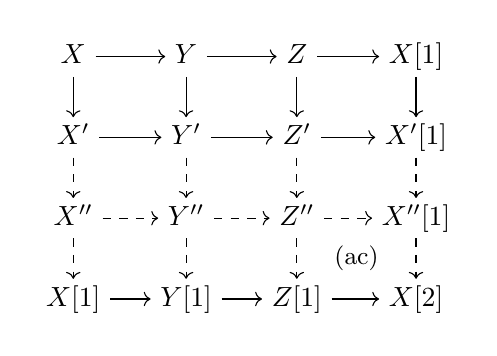
\begin{tikzpicture}[ampersand replacement=\&]
    \matrix(m)[matrix of math nodes, row sep=1.5em, column sep=1.5em,
    text height=1.5ex, text depth=0.25ex]{
      X \& Y \& Z \& X[1] \\
      X' \& Y' \& Z' \& X'[1] \\
      X'' \& Y'' \& Z'' \& X''[1] \\
      X[1]  \& Y[1]  \& Z[1]  \& X[2]\\};

    \path[->] (m-1-1) edge (m-1-2);
    \path[->] (m-1-2) edge (m-1-3);
    \path[->] (m-1-3) edge (m-1-4);

    \path[->] (m-2-1) edge (m-2-2);
    \path[->] (m-2-2) edge (m-2-3);
    \path[->] (m-2-3) edge (m-2-4);

    \path[dashed,->] (m-3-1) edge (m-3-2);
    \path[dashed,->] (m-3-2) edge (m-3-3);
    \path[dashed,->] (m-3-3) edge (m-3-4);

    \path[->] (m-4-1) edge (m-4-2);
    \path[->] (m-4-2) edge (m-4-3);
    \path[->] (m-4-3) edge (m-4-4);

    \path[->] (m-1-1) edge (m-2-1);
    \path[->] (m-1-2) edge (m-2-2);
    \path[->] (m-1-3) edge (m-2-3);
    \path[->] (m-1-4) edge (m-2-4);

    \path[dashed,->] (m-2-1) edge (m-3-1);
    \path[dashed,->] (m-2-2) edge (m-3-2);
    \path[dashed,->] (m-2-3) edge (m-3-3);
    \path[dashed,->] (m-2-4) edge (m-3-4);

    \path[dashed,->] (m-3-1) edge (m-4-1);
    \path[dashed,->] (m-3-2) edge (m-4-2);
    \path[dashed,->] (m-3-3) edge (m-4-3);
    \path[dashed,->] (m-3-4) edge (m-4-4);

    \node[font=\small] at ($(m-3-3)!.5!(m-4-4)$) {(ac)};
  \end{tikzpicture}$$
  normally \emph{does not} give a distinguished triangle
  $X'' \to Y'' \to Z'' \to X'' [1]$.
  For a thorough discussion of this issue, see \cite{Neeman-1991}.
\end{remark}

\begin{landscape}
  \begin{figure}
    \[ \begin{tikzcd}[column sep=1em,font=\small]
        \begin{array}{c} R\Gamma_c (G_\RR, U (\CC), \RR (n)) [-2] \\ \oplus \\ R\Gamma_c (G_\RR, U (\CC), \RR (n)) [-1] \end{array} \ar{d}{Reg_{U,n}^\vee [-1] \oplus id}[swap]{\cong} \ar{r} & \begin{array}{c} R\Gamma_c (G_\RR, X (\CC), \RR (n)) [-2] \\ \oplus \\ R\Gamma_c (G_\RR, X (\CC), \RR (n)) [-1] \end{array} \ar{d}{Reg_{X,n}^\vee [-1] \oplus id}[swap]{\cong} \ar{r} & \begin{array}{c} R\Gamma_c (G_\RR, Z (\CC), \RR (n)) [-2] \\ \oplus \\ R\Gamma_c (G_\RR, Z (\CC), \RR (n)) [-1] \end{array} \ar{d}{Reg_{Z,n}^\vee [-1] \oplus id}[swap]{\cong} \ar{r} & \begin{array}{c} R\Gamma_c (G_\RR, U (\CC), \RR (n)) [-1] \\ \oplus \\ R\Gamma_c (G_\RR, U (\CC), \RR (n)) \end{array} \ar{d}{Reg_{U,n}^\vee \oplus id}[swap]{\cong} \\
        \begin{array}{c} \RHom (R\Gamma (U_\et, \ZZ^c (n)), \RR) [-1] \\ \oplus \\ R\Gamma_c (G_\RR, U (\CC), \RR (n)) [-1] \end{array} \ar{d}{\text{split}}[swap]{\cong} \ar{r} & \begin{array}{c} \RHom (R\Gamma (X_\et, \ZZ^c (n)), \RR) [-1] \\ \oplus \\ R\Gamma_c (G_\RR, X (\CC), \RR (n)) [-1] \end{array} \ar{d}{\text{split}}[swap]{\cong} \ar{r} & \begin{array}{c} \RHom (R\Gamma (Z_\et, \ZZ^c (n)), \RR) [-1] \\ \oplus \\ R\Gamma_c (G_\RR, Z (\CC), \RR (n)) [-1] \end{array} \ar{d}{\text{split}}[swap]{\cong} \ar{r} & \begin{array}{c} \RHom (R\Gamma (U_\et, \ZZ^c (n)), \RR) \\ \oplus \\ R\Gamma_c (G_\RR, U (\CC), \RR (n)) \end{array} \ar{d}{\text{split}}[swap]{\cong} \\
        R\Gamma_\Wc (U, \RR (n)) \ar{r} & R\Gamma_\Wc (X, \RR (n)) \ar{r} & R\Gamma_\Wc (Z, \RR (n)) \ar{r} & R\Gamma_\Wc (U, \RR (n)) [1]
      \end{tikzcd} \]

    \caption{A diagram induced by a closed-open decomposition
      $Z \not\hookrightarrow X \hookleftarrow U$}
    \label{fig:Regulators-and-closed-open-decompositions}
  \end{figure}
\end{landscape}

\begin{lemma}
  \label{lemma:lambda-and-affine-bundles}
  For $n < 0$ and $r \ge 0$, let $X$ be an arithmetic scheme satisfying
  $\mathbf{L}^c (X_\et,n-r)$ and $\mathbf{B} (X,n-r)$. Then there is a natural
  quasi-isomorphism of complexes
  \begin{equation}
    \label{eqn:RGamma-Wc-and-affine-bundles}
    R\Gamma_\Wc (\AA^r_X, \ZZ (n)) \cong R\Gamma_\Wc (X, \ZZ (n-r)) [-2r],
  \end{equation}
  which after passing to the determinants makes the following diagram commute:
  \begin{equation}
    \label{eqn:lambda-and-affine-bundles}
    \begin{tikzcd}[column sep=0.5em]
    & \RR\ar{dl}{\cong}[swap]{\lambda_{\AA^r_X,n}}\ar{dr}{\lambda_{X,n-r}}[swap]{\cong} \\
      (\det_\ZZ R\Gamma_\Wc (\AA^r_X, \ZZ (n)))\otimes \RR \ar{rr}{\cong} & & (\det_\ZZ R\Gamma_\Wc (X, \ZZ (n-r)))\otimes \RR
    \end{tikzcd}
  \end{equation}

  \begin{proof}
    We refer to figure~\ref{fig:RGamma-Wc-and-affine-bundles} below (page
    \pageref{fig:RGamma-Wc-and-affine-bundles}) that shows how the flat morphism
    $p\colon \AA^r_X \to X$ induces the desired quasi-isomorphism
    \eqref{eqn:RGamma-Wc-and-affine-bundles}. Everything comes down to the
    homotopy property of motivic cohomology, namely the fact that $p$ induces a
    quasi-isomorphism
    \[ p^*\colon R\Gamma (X_\et, \ZZ^c (n-r)) [2r] \xrightarrow{\cong}
      R\Gamma (\AA^r_{X,\et}, \ZZ^c (n)) \]
    ---for this see e.g. \cite[Lemma~5.11]{Morin-2014}.
    After passing to real coefficients, we obtain the following diagram:
    \[ \begin{tikzcd}[column sep=1em, font=\small]
        \begin{array}{c} R\Gamma_c (G_\RR, \AA^r_X (\CC), \RR (n)) [-2] \\ \oplus \\ R\Gamma_c (G_\RR, \AA^r_X (\CC), \RR (n)) [-1] \end{array} \ar{d}{Reg_{\AA^r_X,n}^\vee [-1] \oplus id}[swap]{\cong} \ar{r}{\cong} & \begin{array}{c} R\Gamma_c (G_\RR, X (\CC), \RR (n-r)) [-2] [-2r] \\ \oplus \\ R\Gamma_c (G_\RR, X (\CC), \RR (n-r)) [-1] [-2r] \end{array} \ar{d}{Reg_{X,n-r}^\vee [-1] [-2r] \oplus id}[swap]{\cong} \\
        \begin{array}{c} \RHom (R\Gamma (\AA^r_{X,\et}, \ZZ^c (n)), \RR) [-1] \\ \oplus \\ R\Gamma_c (G_\RR, \AA^r_X (\CC), \RR (n)) [-1] \end{array} \ar{d}{\text{split}}[swap]{\cong} \ar{r}{\cong} & \begin{array}{c} \RHom (R\Gamma (X_\et, \ZZ^c (n-r)) [2r], \RR) [-1] \\ \oplus \\ R\Gamma_c (G_\RR, X (\CC), \RR (n-r)) [-1] [-2r] \end{array} \ar{d}{\text{split}}[swap]{\cong} \\
        R\Gamma_\Wc (\AA^r_X, \RR (n)) \ar{r}{\cong} & R\Gamma_\Wc (X, \RR (n-r)) [-2r]
      \end{tikzcd} \]
    Here the first square commutes by the compatibility of the regulator with
    affine bundles (Lemma~\ref{lemma:compatibility-of-B(X,n)}), and the second
    square commutes because the quasi-isomorphism
    \eqref{eqn:RGamma-Wc-and-affine-bundles} gives compatible splittings
    (again, see figure~\ref{fig:RGamma-Wc-and-affine-bundles} below).
    Taking the determinants, we obtain the desired commutative diagram
    \eqref{eqn:lambda-and-affine-bundles}.
  \end{proof}
\end{lemma}

\begin{theorem}
  \label{thm:compatibility-of-C(X,n)}
  For an arithmetic scheme $X$ and $n < 0$, assume $\mathbf{L}^c (X_\et,n)$,
  $\mathbf{B} (X,n)$, and the meromorphic continuation of $\zeta (X,s)$ around
  $s = n$.

  \begin{enumerate}
  \item[1)] If $X = \coprod_{1 \le i \le r} X_i$ is a finite disjoint union of
    arithmetic schemes, then
    $$\mathbf{C} (X,n) \iff \mathbf{C} (X_i,n)\text{ for all }i.$$

  \item[2)] For a closed-open decomposition
    $Z \not\hookrightarrow X \hookleftarrow U$, if two out of three conjectures
    \[ \mathbf{C} (X,n), \quad
      \mathbf{C} (Z,n), \quad
      \mathbf{C} (U,n) \]
    hold, then the third holds as well.

  \item[3)] For any $r \ge 0$, one has
    $$\mathbf{C} (\AA^r_X, n) \iff \mathbf{C} (X, n-r).$$
  \end{enumerate}

  \begin{proof}
    Follows from the previous lemmas
    \ref{lemma:lambda-and-disjoint-unions},
    \ref{lemma:lambda-and-closed-open-decompositions},
    \ref{lemma:lambda-and-affine-bundles},
    together with the respective identities for zeta functions
    \eqref{eqn:zeta-function-for-disjoint-unions},
    \eqref{eqn:zeta-function-for-closed-open-decompositions},
    \eqref{eqn:zeta-function-for-affine-space}.
  \end{proof}
\end{theorem}

\begin{remark}
  As a formal consequence of compatibility with closed-open decompositions, if
  we apply it to the canonical closed embedding $X_\red \hookrightarrow X$,
  then we conclude that
  $R\Gamma_\Wc (X, \ZZ(n)) \cong R\Gamma_\Wc (X_\red, \ZZ(n))$. This is not
  surprising, because Weil-\'{e}tale complexes are constructed from a variant of
  cycle complexes / higher Chow groups, and these do not distinguish $X$ from
  $X_\red$ (unlike, for instance, algebraic $K$-groups).

  This is actually the desired behavior for us, since neither the zeta function
  does: $\zeta (X,s) = \zeta (X_\red,s)$.
\end{remark}

\begin{remark}
  If $X/\FF_q$ is a variety over a finite field, then the proof of
  Theorem~\ref{thm:compatibility-of-C(X,n)} simplifies drastically: we can work
  with the formula \eqref{eqn:special-value-for-X/Fq}, and the following
  properties of motivic cohomology:
  \begin{enumerate}
  \item[1)] $R\Gamma (\coprod_i X_{i,\et}, \ZZ^c (n)) \cong
    \bigoplus_i R\Gamma (X_{i,\et}, \ZZ^c (n))$;

  \item[2)] triangles
    \[ R\Gamma (Z_\et, \ZZ^c (n)) \to
      R\Gamma (X_\et, \ZZ^c (n)) \to
      R\Gamma (U_\et, \ZZ^c (n)) \to
      R\Gamma (Z_\et, \ZZ^c (n))[1] \]
    associated to closed-open decompositions;

  \item[3)] homotopy invariance
    $R\Gamma (X_\et, \ZZ^c (n-r)) [2r] \cong
    R\Gamma (\AA^r_{X,\et}, \ZZ^c (n))$.
  \end{enumerate}
  There are no regulators involved in this case, so we do not need the technical
  lemmas
  \ref{lemma:lambda-and-disjoint-unions},
  \ref{lemma:lambda-and-closed-open-decompositions},
  \ref{lemma:lambda-and-affine-bundles}.
\end{remark}

Considering the projective space $\PP_X^r = \PP_\ZZ^r \times X$,
we have a formula for the zeta function
\begin{equation}
  \label{eqn:zeta-function-for-projective-space}
  \zeta (\PP_X^r, s) = \prod_{0 \le i \le r} \zeta (X, s-i).
\end{equation}

\begin{corollary}[projective bundles]
  Let $X$ be an arithmetic scheme, $n < 0$, and $r \ge 0$.
  For $i = 0,\ldots,r$ assume Conjectures $\mathbf{L}^c (X_\et,n-i)$,
  $\mathbf{B} (X,n-i)$, and meromorphic continuation of $\zeta (X,s)$ around
  $s = n-i$. Then
  \[ \mathbf{C} (X,n-i)\text{ for }i = 0,\ldots,r \Longrightarrow
    \mathbf{C} (\PP_X^r, n). \]

  \begin{proof}
    Applied to the closed-open decomposition
    $\PP_X^{r-1} \not\hookrightarrow \PP_X^r \hookleftarrow \AA_X^r$,
    Theorem~\ref{thm:compatibility-of-C(X,n)} gives
    \[ \mathbf{C} (X, n-r) \text{ and } \mathbf{C} (\PP_X^{r-1}, n)
      \Longrightarrow
      \mathbf{C} (\AA_X^r, n) \text{ and } \mathbf{C} (\PP_X^{r-1}, n)
      \Longrightarrow
      \mathbf{C} (\PP_X^r,n). \]
    The claim follows by induction on $r$.
    (Note that the same inductive argument proves the formula
    \eqref{eqn:zeta-function-for-projective-space} from
    \eqref{eqn:zeta-function-for-affine-space}.)
    \end{proof}
\end{corollary}

\begin{landscape}
  \begin{figure}
    \[ \begin{tikzcd}[font=\small]
        &[2em] &[-2.5em] &[-2.5em] &[-2.5em] R\Gamma_\Wc (U, \ZZ (n))\ar{dl} &[-2.5em] \\
        {[R\Gamma (U_\et, \ZZ^c (n)), \QQ[-2]]} \ar{r}{\alpha_{U,n}}\ar{dd} & R\Gamma_c (U_\et, \ZZ (n)) \ar{dr}{u_\infty} \ar{dd} \ar{rr} & & R\Gamma_\fg (U, \ZZ (n))\ar{dl}[swap]{i_\infty} \ar[dashed]{dd}{\exists!} \ar[crossing over]{rr} & & {[R\Gamma (U_\et, \ZZ^c (n)), \QQ[-1]]} \ar{dd} \\
        & & R\Gamma_c (G_\RR, U (\CC), \ZZ (n)) & & R\Gamma_\Wc (X, \ZZ (n))\ar{dl} \\
        {[R\Gamma (X_\et, \ZZ^c (n)), \QQ[-2]]} \ar{r}{\alpha_{X,n}}\ar{dd} & R\Gamma_c (X_\et, \ZZ (n)) \ar{dr}{u_\infty} \ar{dd} \ar{rr} & & R\Gamma_\fg (X, \ZZ (n)) \ar{dl}[swap]{i_\infty} \ar[dashed]{dd}{\exists!} \ar[crossing over]{rr} & & {[R\Gamma (X_\et, \ZZ^c (n)), \QQ[-1]]} \ar{dd} \\
        & & R\Gamma_c (G_\RR, X (\CC), \ZZ (n)) \ar[<-,near end,crossing over]{uu} & & R\Gamma_\Wc (Z, \ZZ (n))\ar{dl} \\
        {[R\Gamma (Z_\et, \ZZ^c (n)), \QQ[-2]]} \ar{r}{\alpha_{Z,n}}\ar{dd} & R\Gamma_c (Z_\et, \ZZ (n)) \ar{dr}{u_\infty} \ar{dd} \ar{rr} & & R\Gamma_\fg (Z, \ZZ (n)) \ar{dl}[swap]{i_\infty} \ar[dashed]{dd}{\exists!} \ar[crossing over]{rr} & & {[R\Gamma (Z_\et, \ZZ^c (n)), \QQ[-1]]} \ar{dd} \\
        & & R\Gamma_c (G_\RR, Z (\CC), \ZZ (n)) \ar[<-,near end,crossing over]{uu} & & R\Gamma_\Wc (U, \ZZ (n)) [1]\ar{dl} \\
        {[R\Gamma (U_\et, \ZZ^c (n)), \QQ[-1]]} \ar{r}{\alpha_{U,n} [1]} & R\Gamma_c (U_\et, \ZZ (n)) [1] \ar{dr}{u_\infty} \ar{rr} & & R\Gamma_\fg (U, \ZZ (n)) [1] \ar{dl}[swap]{i_\infty [1]} \ar{rr} & & {[R\Gamma (U_\et, \ZZ^c (n)), \QQ]} \\
        & & R\Gamma_c (G_\RR, U (\CC), \ZZ (n)) [1] \ar[<-,near end,crossing over]{uu} \\
      \end{tikzcd} \]

    \caption{Diagram induced by a closed-open decomposition
      $Z \not\hookrightarrow X \hookleftarrow U$}
    \label{fig:RGamma-Wc-and-closed-open-decompositions}
  \end{figure}
\end{landscape}

\begin{landscape}
  \begin{figure}
    \[ \begin{tikzcd}[font=\small]
        &[2em] &[-2.5em] &[-2.5em] &[-2.5em] R\Gamma_\Wc (U, \QQ (n))\ar{dl}\ar{dd} &[-2.5em] \\
        {[R\Gamma (U_\et, \ZZ^c (n)), \QQ[-2]]} \ar{r}\ar{dd} & 0 \ar{dr} \ar{dd} \ar{rr} & & R\Gamma_\fg (U, \QQ (n))\ar{dl}[swap]{0} \ar[dashed]{dd}{\exists!} \ar[crossing over,near start]{rr}{\cong} & & {[R\Gamma (U_\et, \ZZ^c (n)), \QQ[-1]]} \ar{dd} \\
        & & R\Gamma_c (G_\RR, U (\CC), \QQ (n)) & & R\Gamma_\Wc (X, \QQ (n))\ar{dl}\ar{dd} \\
        {[R\Gamma (X_\et, \ZZ^c (n)), \QQ[-2]]} \ar{r}\ar{dd} & 0 \ar{dr} \ar{dd} \ar{rr} & & R\Gamma_\fg (X, \QQ (n)) \ar{dl}[swap]{0} \ar[dashed]{dd}{\exists!} \ar[crossing over,near start]{rr}{\cong} & & {[R\Gamma (X_\et, \ZZ^c (n)), \QQ[-1]]} \ar{dd} \\
        & & R\Gamma_c (G_\RR, X (\CC), \QQ (n)) \ar[<-,near end,crossing over]{uu} & & R\Gamma_\Wc (Z, \QQ (n))\ar{dl}\ar{dd} \\
        {[R\Gamma (Z_\et, \ZZ^c (n)), \QQ[-2]]} \ar{r}\ar{dd} & 0 \ar{dr} \ar{dd} \ar{rr} & & R\Gamma_\fg (Z, \QQ (n)) \ar{dl}[swap]{0} \ar[dashed]{dd}{\exists!} \ar[crossing over,near start]{rr}{\cong} & & {[R\Gamma (Z_\et, \ZZ^c (n)), \QQ[-1]]} \ar{dd} \\
        & & R\Gamma_c (G_\RR, Z (\CC), \QQ (n)) \ar[<-,near end,crossing over]{uu} & & R\Gamma_\Wc (U, \QQ (n)) [1]\ar{dl} \\
        {[R\Gamma (U_\et, \ZZ^c (n)), \QQ[-1]]} \ar{r} & 0 \ar{dr} \ar{rr} & & R\Gamma_\fg (U, \QQ (n)) [1] \ar{dl}[swap]{0} \ar{rr}{\cong} & & {[R\Gamma (U_\et, \ZZ^c (n)), \QQ]} \\
        & & R\Gamma_c (G_\RR, U (\CC), \QQ (n)) [1] \ar[<-,near end,crossing over]{uu} \\
      \end{tikzcd} \]

    \caption{Diagram induced by a closed-open decomposition
      $Z \not\hookrightarrow X \hookleftarrow U$, tensored with $\QQ$}
    \label{fig:RGamma-Wc-and-closed-open-decompositions-otimes-Q}
  \end{figure}
\end{landscape}

\begin{landscape}
  \begin{figure}
    \[ \begin{tikzcd}[font=\small,column sep=1em]
        &[2.75em] &[-2.5em] &[-2.5em] &[-2.5em] R\Gamma_\Wc (\AA^r_X, \ZZ (n))\ar{dl}\ar[dashed,near start]{dd}{\cong} &[-2.5em] \\
        {[R\Gamma (\AA^r_{X,\et}, \ZZ^c (n)), \QQ[-2]]} \ar{r}{\alpha_{\AA^r_X,n}}\ar{dd}{(p^*)^\vee}[swap]{\cong} & R\Gamma_c (\AA^r_{X,\et}, \ZZ (n)) \ar{dr}{u_\infty} \ar{dd}{p_*}[swap]{\cong} \ar{rr} & & R\Gamma_\fg (\AA^r_X, \ZZ (n))\ar{dl}[swap]{i_\infty} \ar[dashed]{dd}{\cong} \ar[crossing over]{rr} & & {[+1]} \ar{dd}{\cong} \\
        & & R\Gamma_c (G_\RR, \AA^r_X (\CC), \ZZ (n)) & & R\Gamma_\Wc (X, \ZZ (n-r)) [-2r]\ar{dl} \\
        {[R\Gamma (X_\et, \ZZ^c (n-r)) [2r], \QQ[-2]]} \ar{r}{\alpha_{X,n-r} [-2r]} & R\Gamma_c (X_\et, \ZZ (n-r)) [-2r] \ar{dr}{u_\infty} \ar{rr} & & R\Gamma_\fg (X, \ZZ (n-r)) [-2r] \ar{dl}[swap]{i_\infty} \ar{rr} & & {[+1]} \\
        & & R\Gamma_c (G_\RR, X (\CC), \ZZ (n-r)) [-2r] \ar[<-,near end,crossing over]{uu}[swap]{p_*}{\cong}\\
        & & \otimes \QQ = \\
        & & & & R\Gamma_\Wc (\AA^r_X, \QQ (n))\ar{dl}\ar[dashed,near start]{dd}{\cong} & \\
        {[R\Gamma (\AA^r_{X,\et}, \ZZ^c (n)), \QQ[-2]]} \ar{r}\ar{dd}{(p^*)^\vee}[swap]{\cong} & 0 \ar{dr} \ar{dd} \ar{rr} & & R\Gamma_\fg (\AA^r_X, \QQ (n))\ar{dl}[swap]{0} \ar[dashed]{dd}{\cong} \ar[crossing over]{rr} & & {[+1]} \ar{dd}{\cong} \\
        & & R\Gamma_c (G_\RR, \AA^r_X (\CC), \QQ (n)) & & R\Gamma_\Wc (X, \QQ (n-r)) [-2r]\ar{dl} \\
        {[R\Gamma (X_\et, \ZZ^c (n-r)) [2r], \QQ[-2]]} \ar{r} & 0 \ar{dr} \ar{rr} & & R\Gamma_\fg (X, \QQ (n-r)) [-2r] \ar{dl}[swap]{0} \ar{rr} & & {[+1]} \\
        & & R\Gamma_c (G_\RR, X (\CC), \QQ (n-r)) [-2r] \ar[<-,near end,crossing over]{uu}[swap]{p_*}{\cong}
      \end{tikzcd} \]

    \caption{Isomorphism
      $R\Gamma_\Wc (\AA^r_X, \ZZ (n)) \cong R\Gamma_\Wc (X, \ZZ (n-r)) [-2r]$
      and its splitting after tensoring with $\QQ$}
    \label{fig:RGamma-Wc-and-affine-bundles}
  \end{figure}
\end{landscape}

%%%%%%%%%%%%%%%%%%%%%%%%%%%%%%%%%%%%%%%%%%%%%%%%%%%%%%%%%%%%%%%%%%%%%%%%%%%%%%%%

\section{Unconditional results}
\label{sec:unconditional-results}

Now we apply Theorem~\ref{thm:compatibility-of-C(X,n)} from the previous section
in order to prove the main theorem stated in the introduction: the validity of
$\mathbf{VO} (X,n)$ and $\mathbf{C} (X,n)$ for all $n < 0$ for cellular schemes
over certain $1$-dimensional bases. In fact, we will construct an even bigger
class of schemes $\mathcal{C} (\ZZ)$ whose elements satisfy the conjectures.
This approach is motivated by \cite[\S 5]{Morin-2014}.

\begin{definition}
  Let $\mathcal{C} (\ZZ)$ be the full subcategory of the category of arithmetic
  schemes generated by the following objects:
  \begin{itemize}
  \item the empty scheme $\emptyset$,
  \item $\Spec \FF_q$ for a finite field,
  \item $\Spec \mathcal{O}_F$ for an abelian number field $F/\QQ$,
  \item curves over finite fields $C/\FF_q$,
  \end{itemize}
  and the following operations.
  \begin{enumerate}
  \item[$\mathcal{C}0)$] $X$ lies in $\mathcal{C} (\ZZ)$ if and only if $X_\red$
    lies in $\mathcal{C} (\ZZ)$.

  \item[$\mathcal{C}1)$] A finite disjoint union $\coprod_{1 \le i \le r} X_i$
    lies in $\mathcal{C} (\ZZ)$ if and only if each $X_i$ lies in
    $\mathcal{C} (\ZZ)$.

  \item[$\mathcal{C}2)$] Let $Z \not\hookrightarrow X \hookleftarrow U$ be a
    closed-open decomposition such that
    $Z_{\red,\CC}$, $X_{\red,\CC}$, $U_{\red,\CC}$ are smooth and
    quasi-projective. Then if two out of three schemes $Z,X,U$ lie in
    $\mathcal{C} (\ZZ)$, then the third lies as well.

  \item[$\mathcal{C}3)$] If $X$ lies in $\mathcal{C} (\ZZ)$, then the affine
    space $\AA^r_X$ also lies in $\mathcal{C} (\ZZ)$ for each $r \ge 0$.
  \end{enumerate}
\end{definition}

We recall that the condition that $X_{\red,\CC}$ is smooth and quasi-projective
is needed to ensure that the regulator morphism exists
(see Remark~\ref{rmk:regulator-is-defined-for-XC-smooth-quasi-proj}).

\begin{proposition}
  \label{prop:C(X,n)-holds-for-C(Z)}
  Conjectures $\mathbf{VO} (X,n)$ and $\mathbf{C} (X,n)$ hold for any
  $X \in \mathcal{C} (\ZZ)$ and $n < 0$.

  \begin{proof}
    Finite fields satisfy $\mathbf{C} (X,n)$ by
    Example~\ref{example:C(X,n)-for-Spec-Fq}.

    If $X = \Spec \mathcal{O}_F$ for an abelian number field $F/\QQ$, then
    Conjecture~$\mathbf{C} (X,n)$ is equivalent to the conjecture of Flach and
    Morin \cite[Conjecture~5.12]{Flach-Morin-2018}, which holds unconditionally
    in this particular case, via reduction to the Tamagawa number conjecture;
    see \cite[\S 5.8.3]{Flach-Morin-2018}, in particular
    [ibid., Proposition~5.35]. The condition $\mathbf{VO} (X,n)$ is also true in
    this case (see Example~\ref{example:VO(X,n)-for-number-rings}).

    If $X = C/\FF_q$ is a curve over a finite field, then $\mathbf{C} (X,n)$
    holds thanks to
    Theorem~\ref{thm:C(X,n)-over-finite-fields}.
    Conjecture~$\mathbf{L}^c (X_\et,n)$ for curves is known and essentially goes
    back to Soul\'{e}; see for instance \cite[Proposition~4.3]{Geisser-2017}.

    Then the fact that the Conjectures $\mathbf{L}^c (X_\et,n)$,
    $\mathbf{B} (X,n)$, $\mathbf{VO} (X,n)$, $\mathbf{C} (X,n)$ are closed under
    the operations $\mathcal{C}1)$--$\mathcal{C}3)$ is
    Lemma~\ref{lemma:compatibility-of-Lc(X,n)},
    Lemma~\ref{lemma:compatibility-of-B(X,n)},
    Proposition~\ref{prop:compatibility-of-VO(X,n)},
    and Theorem~\ref{thm:compatibility-of-C(X,n)}
    respectively.
  \end{proof}
\end{proposition}

\begin{lemma}
  Any $0$-dimensional arithmetic scheme $X$ lies in $\mathcal{C} (\ZZ)$.

  \begin{proof}
    Since $X$ is a noetherian scheme of dimension $0$, it is a finite disjoint
    union of $\Spec A_i$ for some artinian local rings $A_i$. Thanks to
    $\mathcal{C}1)$, we can assume that $X = \Spec A$, and thanks to
    $\mathcal{C}0)$, we can assume that $X$ is reduced. But then $A = k$ is a
    field. Since $X$ is a scheme of finite type over $\Spec \ZZ$, we conclude
    that $X = \Spec \FF_q \in \mathcal{C} (\ZZ)$.
  \end{proof}
\end{lemma}

\begin{proposition}
  \label{prop:particular-cases-1-dim-base}
  Let $B$ be a $1$-dimensional arithmetic scheme. Assume that each of the
  generic points $\eta \in B$ satisfies one of the following properties:
  \begin{enumerate}
  \item[a)] $\fchar \kappa (\eta) = p > 0$;

  \item[b)] $\fchar \kappa (\eta) = 0$, and $\kappa (\eta)/\QQ$ is an abelian
    number field.
  \end{enumerate}
  Then $B \in \mathcal{C} (\ZZ)$.

  \begin{proof}
    We will see that such a scheme can be obtained from $\Spec \mathcal{O}_F$
    for an abelian number field $F/\QQ$, or a curve over a finite field
    $C/\FF_q$, using the operations $\mathcal{C}0)$, $\mathcal{C}1)$,
    $\mathcal{C}2)$ that appear in the definition of $\mathcal{C} (\ZZ)$.

    Thanks to $\mathcal{C}0)$, we can assume that $B$ is reduced. Consider the
    normalization $\nu\colon B' \to B$. This is a birational morphism, and there
    exist open dense subsets $U' \subseteq B'$ and $U \subseteq B$ such that
    $\left.\nu\right|_{U'}\colon U' \xrightarrow{\cong} U$. Now $B\setminus U$
    is $0$-dimensional, and therefore $B\setminus U \in \mathcal{C} (\ZZ)$ by
    the previous lemma. Thanks to $\mathcal{C}2)$, it is enough to check that
    $U' \in \mathcal{C} (\ZZ)$, and this would imply $B \in \mathcal{C} (\ZZ)$.

    Now $U'$ is a finite disjoint union of normal integral schemes, so by
    $\mathcal{C}1)$ we can assume that $U'$ is integral. Consider the generic
    point $\eta \in U'$ and the residue field $F = \kappa (\eta)$. There are two
    distinct cases to consider.

    \begin{enumerate}
    \item[a)] If $\fchar F = p > 0$, then $U'$ is a curve over a finite field,
      so it lies in $\mathcal{C} (\ZZ)$ by the definition.

    \item[b)] If $\fchar F = 0$, then by our assumptions, $F/\QQ$ is an abelian
      number field.

      We note that if $V' \subseteq U'$ is an affine open neighborhood of
      $\eta$, then $U'\setminus V' \in \mathcal{C} (\ZZ)$ by the previous
      lemma. Therefore, we can assume without loss of generality that $U'$ is
      affine.

      We have $U' = \Spec \mathcal{O}$, where $\mathcal{O}$ is a finitely
      generated integrally closed domain. All this means that
      $\mathcal{O}_F \subseteq \mathcal{O} = \mathcal{O}_{F,S}$ for some finite
      set $S$. Now $U' = \Spec \mathcal{O}_F \setminus S$, and
      $S \in \mathcal{C} (\ZZ)$, so again, everything reduces to the case of
      $U' = \Spec \mathcal{O}_F$, which lies in $\mathcal{C} (\ZZ)$ by the
      definition. \qedhere
    \end{enumerate}
  \end{proof}
\end{proposition}

\begin{remark}
  Schemes as above were considered by Jordan and Poonen in
  \cite{Jordan-Poonen-2020}, where the authors write down a special value
  formula at $s = 1$, generalizing the classical class number formula. Namely,
  they consider the case of $B$ reduced and affine, albeit without requiring
  $\kappa (\eta)/\QQ$ to be abelian.
\end{remark}

\begin{example}
  If $B = \Spec \mathcal{O}$ for a nonmaximal order
  $\mathcal{O} \subset \mathcal{O}_F$, where $F/\QQ$ is an abelian number field,
  then our formalism gives a cohomological interpretation of the special values
  of $\zeta_\mathcal{O} (s)$ at $s = n < 0$. This already seems to be a new
  result.
\end{example}

\begin{definition}
  \label{dfn:B-cellular-scheme}
  Let $X \to B$ be a $B$-scheme. We say that $X$ is \textbf{$B$-cellular} if it
  admits a filtration by closed subschemes
  \begin{equation}
    \label{eqn:cellular-decomposition}
    X = Z_N \supseteq Z_{N-1} \supseteq \cdots \supseteq Z_0 \supseteq Z_{-1} = \emptyset
  \end{equation}
  such that $Z_i\setminus Z_{i-1} \cong \coprod_j \AA^{r_{i_j}}_B$ is a finite
  union of affine $B$-spaces.
\end{definition}

For instance, projective spaces $\PP^r_B$ and in general Grassmannians
$\Gr (k,\ell)_B$ are cellular. Many interesting examples of cellular schemes as
above arise from actions of algebraic groups on varieties and
Bia\l{}ynicki-Birula theorem; for this see \cite{Wendt-2010} and
\cite{Brosnan-2005}.

\begin{proposition}
  \label{prop:cellular-schemes-in-C(Z)}
  Let $X$ be a $B$-cellular arithmetic scheme, where $B \in \mathcal{C} (\ZZ)$,
  and $X_{\red,\CC}$ is smooth and quasi-projective. Then
  $X \in \mathcal{C} (\ZZ)$.

  \begin{proof}
    Looking at the corresponding cellular decomposition
    \eqref{eqn:cellular-decomposition}, we better pass to open complements
    $U_i = X\setminus Z_i$, to obtain a filtration
    $$X = U_{-1} \supseteq U_1 \supseteq \cdots \supseteq U_{N-1} \supseteq U_N = \emptyset,$$
    with $U_{i,\CC}$ smooth and quasi-projective, being \emph{open}
    subvarieties in $X_\CC$. Now we have closed-open decompositions
    $\coprod_j \AA^{r_{i,j}}_B \not\hookrightarrow U_i \hookleftarrow U_{i+1}$,    
    and the claim follows by induction on the length of the cellular
    decomposition, using operations
    $\mathcal{C}1)$--$\mathcal{C}3)$.
  \end{proof}
\end{proposition}

As a corollary of the above, we obtain the following result, stated in the
introduction.

\begin{theorem}
  Let $B$ be a $1$-dimensional arithmetic scheme satisfying the assumptions of
  Proposition~\ref{prop:particular-cases-1-dim-base}. If $X$ is a $B$-cellular
  arithmetic scheme with smooth and quasi-projective fiber $X_{\red,\CC}$, then
  Conjectures $\mathbf{VO} (X,n)$ and $\mathbf{C} (X,n)$ hold
  unconditionally for any $n < 0$.

  \begin{proof}
    Follows from propositions
    \ref{prop:C(X,n)-holds-for-C(Z)},
    \ref{prop:particular-cases-1-dim-base},
    \ref{prop:cellular-schemes-in-C(Z)}.
  \end{proof}
\end{theorem}

%%%%%%%%%%%%%%%%%%%%%%%%%%%%%%%%%%%%%%%%%%%%%%%%%%%%%%%%%%%%%%%%%%%%%%%%%%%%%%%%

\begin{appendices}
\section{Determinants of complexes}
\label{app:determinants}

In this appendix we include a brief overview of determinants of complexes.
The original construction is due to Knudsen and Mumford
\cite{Knudsen-Mumford-1976}, and other useful expositions can be found in
\cite[Appendix~A]{Gelfand-Kapranov-Zelevinsky-1994} and
\cite[\S 2.1]{Kato-1993}.

For our purposes, let $R$ be a commutative ring, which is an integral domain
(we will be interested in $R = \ZZ$, $\QQ$, $\RR$). Denote by
$\mathcal{P}_\is (R)$ (``Picard'') the category of graded invertible
$R$-modules. It has as its objects pairs $(L,r)$, where $L$ is an invertible
$R$-module (= projective of rank $1$) and $r \in \ZZ$. The morphisms in this
category are given by
\[ \Hom_{\mathcal{P}_\is (R)} ((L,r), (M,s)) = \begin{cases}
    \Isom_R (L,M), & r = s, \\
    \emptyset, & r \ne s.
  \end{cases} \]
This category is equipped with tensor products
$$(L,r) \otimes_R (M,s) = (L\otimes_R M, r + s)$$
with commutativity isomorphisms
\begin{align*}
  \psi\colon (L,r) \otimes_R (M,s) & \xrightarrow{\cong}
                                     (M,s) \otimes_R (L,r), \\
  \ell \otimes m & \mapsto (-1)^{r\,s}\,m\otimes \ell
\end{align*}
for $\ell \in L$, $m \in M$.

The unit object with respect to this product is $\bone = (R,0)$, and for each
$(L,r) \in \mathcal{P}_\is (R)$ the inverse is given by $(L^{-1}, -r)$ where
$L^{-1} = \iHom_R (L,R)$. The canonical evaluation morphism
$L \otimes_R \iHom_R (L,R) \to R$ induces an isomorphism
$$(L,r) \otimes_R (L^{-1}, -r) \cong \bone.$$

\begin{definition}
  \label{dfn:determinant-of-projective-fg-module}
  We denote by $\mathcal{C}_\is (R)$ the category whose objects are finitely
  generated projective $R$-modules and whose morphisms are isomorphisms.  For
  $A \in \mathcal{C}_\is (R)$ we define the corresponding determinant as an
  object in $\mathcal{P}_\is (R)$ given by
  $$\det_R (A) = \Bigl(\bigwedge^{\rk_R A}_R A, \rk_R A\Bigr).$$
  Here $\rk_R A$ is the rank of $A$, so that the top exterior power
  $\bigwedge^{\rk_R A}_R A$ is an invertible $R$-module.
\end{definition}

This gives a functor $\det_R\colon \mathcal{C}_\is (R) \to \mathcal{P}_\is (R)$.
The main result of \cite[Chapter~I]{Knudsen-Mumford-1976} is that this
construction can be generalized as follows. Let $\mathbf{D} (R)$ be the derived
category of the category of $R$-modules. Recall that a complex $A^\bullet$ is
\textbf{perfect} if it is quasi-isomorphic to a bounded complex of finitely
generated projective $R$-modules. We denote by $\Parf_\is (R)$ the subcategory
of $\mathbf{D} (R)$ whose objects consist of perfect complexes, and whose
morphisms are quasi-isomorphisms of complexes.

\begin{theorem}[Knudsen--Mumford]
  The determinant can be extended to perfect complexes of $R$-modules as
  follows.

  \begin{enumerate}
  \item[I)] For every ring $R$ there exists a functor
    $$\det_R\colon \Parf_\is (R) \to \mathcal{P}_\is (R)$$
    such that $\det_R (0) = \bone$.

  \item[II)] For every short exact sequence of complexes in $\Parf_\is (R)$
    \[ 0 \to A^\bullet \xrightarrow{\alpha} B^\bullet
      \xrightarrow{\beta} C^\bullet \to 0 \]
    there exists an isomorphism
    \[ i_R (\alpha,\beta)\colon
      \det_R A^\bullet \otimes_R \det_R C^\bullet
      \xrightarrow{\cong} \det_R B^\bullet. \]
    In particular, for the short exact sequence
    \[ \begin{tikzcd}[column sep=1em]
        &[-1.5em] 0 \ar{r} & A^\bullet \ar{r}{id} & A^\bullet \ar{r} & 0^\bullet \ar{r} & 0 &[-1.5em] \\[-2em]
        \text{(resp.} & 0 \ar{r} & 0^\bullet \ar{r} & A^\bullet \ar{r}{id} & A^\bullet \ar{r} & 0 & \text{)}
      \end{tikzcd} \]
    the isomorphism $i_R (id,0)$ (resp. $i_R (0,id)$) is the canonical isomorphism
    $$\det_R A^\bullet \otimes_R \bone \xrightarrow{\cong} \det_R A^\bullet$$
  \end{enumerate}

  Moreover, the following properties hold.

  \begin{enumerate}
  \item[i)] Given an isomorphism of short exact sequences of complexes
    \[ \begin{tikzcd}
        0 \ar{r} & A^\bullet \ar{r}{\alpha}\ar{d}{u}[swap]{\cong} & B^\bullet \ar{r}{\beta}\ar{d}{v}[swap]{\cong} & C^\bullet \ar{r}\ar{d}{w}[swap]{\cong} & 0 \\
        0 \ar{r} & A'^\bullet \ar{r}{\alpha'} & B'^\bullet \ar{r}{\beta'} & C'^\bullet \ar{r} & 0
      \end{tikzcd} \]
    the diagram
    \[ \begin{tikzcd}[column sep=5em]
        \det_R A^\bullet \otimes_R \det_R C^\bullet \ar{r}{i^* (\alpha,\beta)}[swap]{\cong}\ar{d}{\det_R (u) \otimes \det_R (w)}[swap]{\cong} & \det_R B^\bullet\ar{d}{\det_R (v)}[swap]{\cong} \\
        \det_R A'^\bullet \otimes_R \det_R C'^\bullet \ar{r}{i^* (\alpha',\beta')}[swap]{\cong} & \det_R B'^\bullet
      \end{tikzcd} \]
    commutes.

  \item[ii)] Given a commutative $3\times 3$ diagram with rows and columns short
    exact sequences
    \[ \begin{tikzcd}[row sep=1em, column sep=1em]
        & 0\ar{d} & 0\ar{d} & 0\ar{d} \\
        0\ar{r} & A^\bullet\ar{r}{\alpha}\ar{d}{u} & B^\bullet\ar{r}{\beta}\ar{d}{u'} & C^\bullet\ar{r}\ar{d}{u''} & 0 \\
        0\ar{r} & A'^\bullet\ar{r}{\alpha'}\ar{d}{v} & B'^\bullet\ar{r}{\beta'}\ar{d}{v'} & C'^\bullet\ar{r}\ar{d}{v''} & 0 \\
        0\ar{r} & A''^\bullet\ar{r}{\alpha''}\ar{d} & B''^\bullet\ar{r}{\beta''}\ar{d} & C''^\bullet\ar{r}\ar{d} & 0 \\
        & 0 & 0 & 0
      \end{tikzcd} \]
    the diagram
    \[ \begin{tikzcd}[column sep=7em]
        \det_R A^\bullet \otimes_R \det_R C^\bullet \otimes_R \det_R A''^\bullet \otimes_R \det_R C''^\bullet \ar{r}{i_R (\alpha,\beta) \otimes i_R (\alpha'',\beta'')}[swap]{\cong}\ar{d}{id \otimes \psi \otimes id}[swap]{\cong} & \det_R B^\bullet \otimes_R \det_R B''^\bullet\ar{dd}{i_R (u',v')}[swap]{\cong} \\
        (\det_R A^\bullet \otimes_R \det_R A''^\bullet) \otimes_R (\det_R C^\bullet \otimes_R \det_R C''^\bullet)\ar{d}[swap]{\cong}{i_R (u,v) \otimes i_R (u'',v'')} \\
        \det_R A'^\bullet \otimes_R \det_R C'^\bullet \ar{r}{i_R (\alpha',\beta')}[swap]{\cong} & \det_R B'^\bullet
      \end{tikzcd} \]
    commutes.

  \item[iii)] $\det$ and $i$ commute with base change. Namely, given a ring
    homomorphism $f\colon R\to S$, there is a natural isomorphism
    \[ \eta_A = \eta_{A^\bullet} (f)\colon
      \det_S (A^\bullet \otimes_R^\mathbf{L} S) \xrightarrow{\cong}
      (\det_R A^\bullet) \otimes_R S, \]
    such that for every short exact sequence of complexes
    \[ 0 \to A^\bullet \xrightarrow{\alpha} B^\bullet \xrightarrow{\beta}
      C^\bullet \to 0 \]
    the diagram
    \[ \begin{tikzcd}[column sep=5em]
        \det_S (A^\bullet \otimes_R^\mathbf{L} S) \otimes_S \det_S (C^\bullet \otimes_R^\mathbf{L} S) \ar{d}{\eta_A \otimes \eta_C}[swap]{\cong}\ar{r}{i_S (\alpha\otimes S, \beta\otimes S)}[swap]{\cong} & \det_S (B^\bullet \otimes_R^\mathbf{L} S) \ar{d}{\eta_B}[swap]{\cong} \\
        \Bigl((\det_R A^\bullet) \otimes_R S\Bigr) \otimes_S \Bigl((\det_R C^\bullet) \otimes_R S\Bigr) \ar{r}{i_R (\alpha,\beta) \otimes S}[swap]{\cong} & (\det_R B^\bullet) \otimes_R S
      \end{tikzcd} \]
    commutes. Similarly, there is compatibility with compositions of base
    changes along $R \xrightarrow{f} S \xrightarrow{g} T$ (we omit the
    corresponding commutative diagram).
  \end{enumerate}
\end{theorem}

\begin{remark}
  We refer to \cite{Knudsen-Mumford-1976} for the actual construction.
  In practice, the following considerations are useful; see [ibid.] for the
  proofs.

  \begin{enumerate}
  \item[1)] If $A^\bullet$ is a bounded complex where each object $A^i$ is
    perfect (i.e. admits a finite length resolution by finitely generated
    projective $R$-modules), then
    $$\det_R A^\bullet \cong \bigotimes_{i\in \ZZ} (\det_R A^i)^{(-1)^i}.$$
    In particular, if each $A^i$ is already a finitely generated projective
    $R$-module, then $\det_R A^i$ in the above formula is given by
    \ref{dfn:determinant-of-projective-fg-module}.

  \item[2)] If the cohomology modules $H^i (A^\bullet)$ are perfect, then
    \[ \det_R A^\bullet \cong
      \bigotimes_{i\in \ZZ} (\det_R H^i (A^\bullet))^{(-1)^i}. \]
  \end{enumerate}
\end{remark}

The determinants also behave well not only with short exact sequences, but with
distinguished triangles.

\begin{proposition}[{\cite[Proposition~7]{Knudsen-Mumford-1976}}]
  \label{prop:det-and-isos-of-triangles}
  For a distinguished triangle of complexes in $\Parf_\is (R)$
  \[ A^\bullet \xrightarrow{u} B^\bullet \xrightarrow{v} C^\bullet
    \xrightarrow{w} A^\bullet [1] \]
  there is a canonical isomorphism
  \[ i_R (u,v,w)\colon \det_R A^\bullet \otimes_R \det_R C^\bullet
    \xrightarrow{\cong} \det_R B^\bullet, \]
  which is functorial in the following sense: given a (quasi-)isomorphism of
  distinguished triangles
  \[ \begin{tikzcd}
      A^\bullet \ar{r}{u}\ar{d}{f}[swap]{\cong} & B^\bullet \ar{r}{v}\ar{d}{g}[swap]{\cong} & C^\bullet \ar{r}{w}\ar{d}{h}[swap]{\cong} & A^\bullet [1]\ar{d}{f[1]}[swap]{\cong} \\
      A'^\bullet \ar{r}{u} & B'^\bullet \ar{r}{v} & C'^\bullet \ar{r}{w} & A'^\bullet [1]
    \end{tikzcd} \]
  the diagram
  \[ \begin{tikzcd}[column sep=5em]
      \det_R A^\bullet \otimes_R \det_R C^\bullet \ar{r}{i_R (u,v,w)}[swap]{\cong}\ar{d}{\det_R (f) \otimes \det_R (h)}[swap]{\cong} & \det_R B^\bullet\ar{d}{\det_R (g)}[swap]{\cong} \\
      \det_R A'^\bullet \otimes_R \det_R C'^\bullet \ar{r}{i_R (u',v',w')}[swap]{\cong} & \det_R B'^\bullet
    \end{tikzcd} \]
  commutes.
\end{proposition}

\begin{remark}
  In what follows, for $(L,r) \in \mathcal{P}_\is (R)$ we will forget about
  $r$ and treat the determinant as an invertible $R$-module.
\end{remark}

A particular very simple case of interest is when all cohomology groups
$H^i (A^\bullet)$ are finite.

\begin{lemma}
  \label{lemma:determinant-for-torsion-cohomology}
  ~

  \begin{enumerate}
  \item[1)] Let $A$ be a finite abelian group. Then
    \[ (\det_\ZZ A) \subset (\det_\ZZ A) \otimes \QQ
      \cong \det_\QQ (A \otimes \QQ) = \det_\QQ (0) \cong \QQ \]
    corresponds to the fractional ideal $\frac{1}{\# A} \ZZ \subset \QQ$.

  \item[2)] In general, let $A^\bullet$ be a perfect complex of abelian groups
    such that the cohomology groups $H^i (A^\bullet)$ are all finite. Then
    $\det_\ZZ A^\bullet$ corresponds to the fractional ideal
    $\frac{1}{m}\,\ZZ \subset \QQ$, where
    $$m = \prod_{i\in \ZZ} |H^i (A^\bullet)|^{(-1)^i}.$$
  \end{enumerate}

  \begin{proof}
    Since $\det_\ZZ (A\oplus B) \cong \det_\ZZ A \otimes \det_\ZZ B$, in
    part 1) it would be enough to consider the case of a cyclic group
    $A = \ZZ/m\ZZ$. Then we have a quasi-isomorphism of complexes
    \[ \ZZ/m\ZZ [0] \cong \Bigl[
      \mathop{m\ZZ}_{\text{deg.\,}-1} \hookrightarrow
      \mathop{\ZZ}_{\text{deg.\,}0}
      \Bigr]. \]
    Therefore,
    $$\det_\ZZ (\ZZ/m\ZZ) \cong \ZZ \otimes (m\ZZ)^{-1} \cong (m\ZZ)^{-1},$$
    which corresponds to $\frac{1}{m}\,\ZZ$ inside $\QQ$.
    Part 2) follows immediately from 1) using the isomorphism
    \[ \det_\ZZ A^\bullet \cong
      \bigotimes_{i\in \ZZ} (\det_\ZZ H^i (A^\bullet))^{(-1)^i}. \qedhere \]
  \end{proof}
\end{lemma}

\begin{remark}
  The above argument works in a more general setting, assuming $R$ is a regular
  noetherian ring and $A$ is a finitely generated torsion $R$-module (replacing
  $\QQ$ with the total quotient field $Q (R)$).
\end{remark}

\end{appendices}

%%%%%%%%%%%%%%%%%%%%%%%%%%%%%%%%%%%%%%%%%%%%%%%%%%%%%%%%%%%%%%%%%%%%%%%%%%%%%%%%

\bibliographystyle{abbrv}
\bibliography{../weil-etale}

\end{document}
